\section{Phân tích phim truyền thông và xã hội}

\subsection{Giới thiệu chung}

Trong những năm gần đây, các nhà phân tích và nhà đầu tư ngày càng quan tâm đến việc đánh giá rủi ro tài chính trong sản xuất phim. Nghiên cứu này sử dụng phân tích hồi quy tuyến tính bội để dự đoán thành công về mặt tài chính của phim và nghiên cứu mối quan hệ giữa số lần chiếu và năm.

\subsection{Phát biểu bài toán}

Mục tiêu chính của phần này là khám phá và phân tích tổng doanh thu của phim trong hai năm 2014 và 2015 cũng như kiểm tra mối quan hệ và ý nghĩa của một số biến giải thích. Hơn nữa, đồ án xây dựng một mô hình hồi quy tối ưu để đưa ra dự đoán về sự thành công về mặt tài chính, tức là tổng doanh thu của một bộ phim trong hai năm 2014 và 2015. 


\subsection{Giới thiệu về dữ liệu}

Bộ dữ liệu phim truyền thông và xã hội (conventional and social media dataset) được sử dụng trong đồ án này có cấu trúc tương đối đơn giản mà một số người có ích kiến thức về phim truyền hình cũng có thể hiểu được. Vấn đề chính của bộ dữ liệu là missing values, và chúng tôi sẽ cố gắng xử lý nó bằng một số kỹ thuật đã biết.

Ngành công nghiệp điện ảnh là một ngành đóng góp đáng kể cho nền kinh tế của một quốc gia và là một nhà tuyển dụng lớn tại Hoa Kỳ. Do chi phí lớn liên quan đến sản xuất phim, các nhà phân tích cần nghiên cứu và hiểu các biến số chính góp phần vào thành công về mặt thương mại và tài chính của một bộ phim. Đồ án có thể cung cấp thông tin chi tiết về các tính năng chính góp phần vào thành công về mặt tài chính của các bộ phim và thúc đẩy nghiên cứu trong tương lai để xem xét mối quan hệ giữa các biến giải thích đặc biệt độc đáo trong tập dữ liệu. Hơn nữa nó còn có thể giúp các nhà sản xuất phim xác định những tính năng nào cần tập trung vào trong giai đoạn quảng bá để cải thiện thành công của bộ phim.


\subsection{Khám phá và tiền xử lý dữ liệu}


\subsubsection{Đọc dữ liệu và một số kiểm tra khởi đầu}

Trước hết, ta đọc dữ liệu

\begin{lstlisting}
# Đọc dữ liệu từ tập tin
raw_data = read_excel("../../data/part1/CSM.xlsx", sheet = 1)
str(raw_data)

# Thay đổi tên biến `Aggregate Followers` thành `AggregateFollowers`
names(raw_data)[names(raw_data) == 'Aggregate Followers'] <- 'AggregateFollowers'
\end{lstlisting}

Dữ liệu này không có hiện tượng trùng lặp. Dựa trên thông tin của tập dữ liệu, ta thấy mỗi dòng mang ý nghĩa khác nhau, tức là mỗi quan trắc độc lập nhau. Ý nghĩa từng cột như sau:
\begin{itemize}
    \item \textbf{Movie}: tên phim
    \item \textbf{Year}: năm phát hành
    \item \textbf{Ratings}: điểm đánh giá
    \item \textbf{Genre}: thể loại phim
    \item \textbf{Gross}: tổng doanh thu
    \item \textbf{Budget}: tổng chi phí
    \item \textbf{Screens}: số rạp chiều
    \item \textbf{Sequel}: phần phim
    \item \textbf{Sentiment}: ý kiến khán giả
    \item \textbf{Views}: số lượt xem
    \item \textbf{Likes}: số lượt thích
    \item \textbf{Dislikes}: số lượt chê
    \item \textbf{Comments}: số bình luận
    \item \textbf{Aggregate Followers}: số người theo dõi
\end{itemize}

Ta thấy biến Dislikes thể hiện ý nghĩa tương tự biến Likes nhưng có chiều hướng ngược lại. Nên ta có thể loại bỏ biến này khỏi tập dữ liệu.

\subsubsection{Các cột với kiểu dữ liệu số phân bố như thế nào?}

Ta kiểm tra một số thông tin thống kê mô tả của bộ dữ liệu

\begin{minted}{R}
# A tibble: 12 × 7
   variable           missing     min      lower     median      upper       max
   <chr>                <dbl>   <dbl>      <dbl>      <dbl>      <dbl>     <dbl>
 1 Year                   0    2014       2014       2014       2015      2.02e3
 2 Ratings                0       3.1        5.8        6.5        7.1    8.7 e0
 3 Gross                  0    2470   10300000   37400000   89350000      6.43e8
 4 Budget                 0.4 70000    9000000   28000000   65000000      2.5 e8
 5 Screens                4.3     2        449       2777       3372      4.32e3
 6 Sequel                 0       1          1          1          1      7   e0
 7 Sentiment              0     -38          0          0          5.5    2.9 e1
 8 Views                  0     698     623302    2409338    5217380.     3.26e7
 9 Likes                  0       1       1776.      6096      15248.     3.71e5
10 Dislikes               0       0        106.       341        698.     1.40e4
11 Comments               0       0        248.       837       2137      3.84e4
12 AggregateFollowers    15.2  1066     183025    1052600    3694500      3.10e7
\end{minted}
Nhận xét:
\begin{itemize}
    \item Có hiện tượng missing values đối với cột AggregateFollowers, Screens và Budget. Cụ thể, ta thấy biến Aggregate Followers có tỷ lệ missing 15.2\%, biến Screens có tỷ lệ 4.3\% và biến Budget có tỷ lệ missing 0.4\%.
    \item  Có những bộ phim không có likes/ dislikes/ comments, ta sẽ loại bỏ những dòng này.
\end{itemize}

\subsubsection{Các cột với kiểu dữ liệu phân loại phân bố như thế nào?}

Khảo sát cột Genre thể hiện các thể loại phim, ta trực quan bằng biểu đổ tròn dưới đây.

\begin{figure}[H]
    \centering
    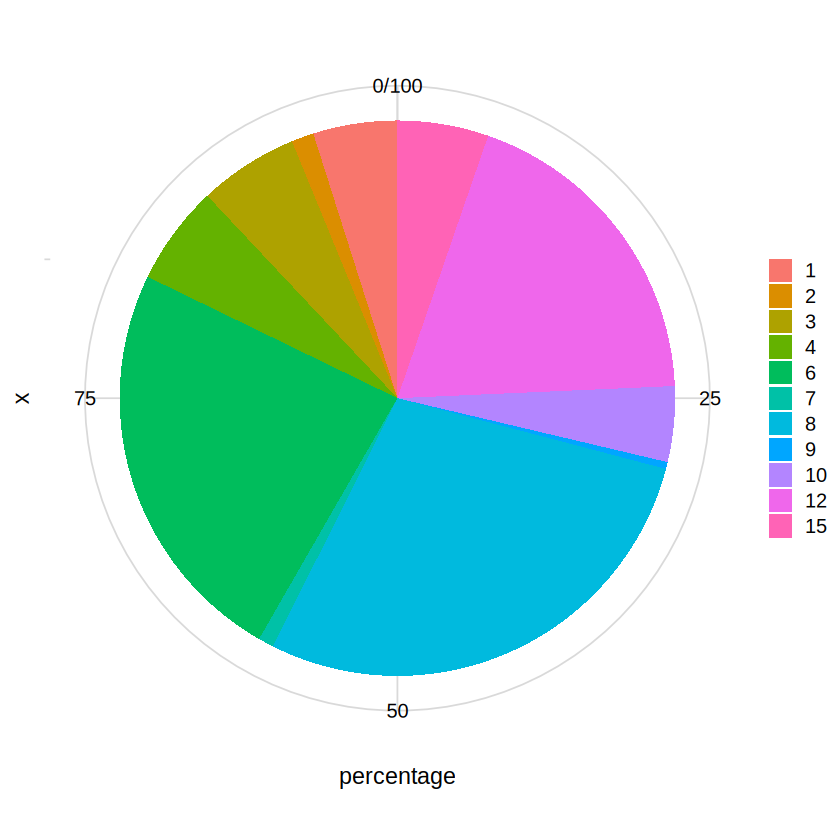
\includegraphics[width=0.75\columnwidth]{csm_figures/genre_part01.png}
    \caption{Tỷ lệ các thể loại phim.}
    \label{fig:genre}
\end{figure}
Nhận xét:
\begin{itemize}
    \item Các thể loại phim phân bố không đều nhau
    \item 
\end{itemize}

\subsubsection{Xử lý dữ liệu bị thiếu}

Trong đồ án này, chúng tôi khảo sát nhiều phương pháp xử lý dữ liệu bị thiếu như sau:
\begin{itemize}
    \item Chèn không (zeros imputed)
    \item Chèn trung bình (means imputed)
    \item Chèn trung vị (median imputed)
    \item Điền các giá trị bị thiếu dựa trên PCA (imputed PCA)
\end{itemize}

Dựa trên kết quả thực nghiệm, chúng tôi chọn điền các giá trị bị thiếu dựa trên PCA vì có kết quả xây dựng mô hình tốt. Chi tiết các kỹ thuật khác được trình bày trong các file code.

Các bước thực hiện điền các giá trị bị thiếu dựa trên PCA:
\begin{itemize}
    \item Bước 1: ước lượng số thành phần chính
\begin{lstlisting}
# Ước lượng thành phần chính
nPCs <- estim_ncpPCA(raw_data[, -c(1)])
print(nPCs)
\end{lstlisting}
    \item Bước 2: điền các giá trị bị thiếu
\begin{lstlisting}
# Xử lý missing value
processed_data <- imputePCA(raw_data[, -c(1)], ncp = nPCs$ncp, scale = TRUE)
processed_data <- processed_data$completeObs
\end{lstlisting}
\end{itemize}

Đánh giá kết quả bằng cách trực quan hóa phân phối trước và sau khi thực hiện việc điền các giá trị bị thiếu:
\begin{lstlisting}
# Trực quan phân phối trước và sau khi fill missing value

h1 <- ggplot(raw_data, aes(x = Budget)) +
  geom_histogram(fill = "#15ad4f", color = "#000000", position = "identity") +
  ggtitle("Budget Original distribution") +
  theme_classic()
h2 <- ggplot(raw_data, aes(x = Screens)) +
  geom_histogram(fill = "#1543ad", color = "#000000", position = "identity") +
  ggtitle("Screens Original distribution") +
  theme_classic()
h3 <- ggplot(raw_data, aes(x = AggregateFollowers )) +
  geom_histogram(fill = "#ad8415", color = "#000000", position = "identity") +
  ggtitle("AggregateFollowers Original distribution") +
  theme_classic()

  
h4 <- ggplot(processed_data, aes(x = Budget)) +
  geom_histogram(fill = "#15ad4f", color = "#000000", position = "identity") +
  ggtitle("Budget PCA-filled distribution") +
  theme_classic()
h5 <- ggplot(processed_data, aes(x = Screens)) +
  geom_histogram(fill = "#1543ad", color = "#000000", position = "identity") +
  ggtitle("Screens PCA-filled distribution") +
  theme_classic()
h6 <- ggplot(processed_data, aes(x = AggregateFollowers )) +
  geom_histogram(fill = "#ad8415", color = "#000000", position = "identity") +
  ggtitle("AggregateFollowers PCA-filled distribution") +
  theme_classic()

plot_grid(h1, h2, h3, h4, h5, h6, nrow = 2, ncol = 3, rel_widths = c(1, 1), rel_heights = c(1, 1))
\end{lstlisting}

\begin{figure}[H]
    \centering
    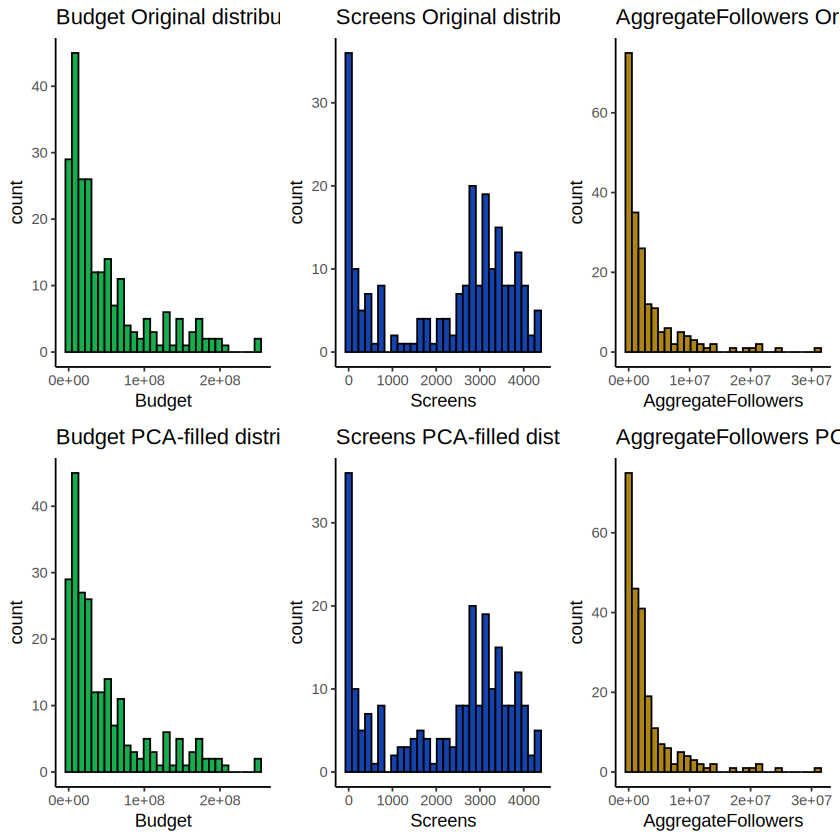
\includegraphics[width=0.75\columnwidth]{csm_figures/imputed_PCA.png}
    \caption{Phân phối trước và sau khi điền các giá trị bị thiếu đối với các cột Budget, Screens và AggregateFollowers.}
    \label{fig:imputed_PCA}
\end{figure}
Nhận xét:
\begin{itemize}
    \item Ta thấy phân phối sau khi điền không có quá nhiều chênh lệch so với phân phối dữ liệu gốc (đã bỏ qua các giá trị bị thiếu)
\end{itemize}

\subsection{Quay lại bước khám phá và tiền xử lý dữ liệu}

Trong phần này, chúng tôi khảo sát các biến để chuẩn hóa dữ liệu. Chúng tôi lựa chọn box-cox transformation để tìm kiếm giá trị $\lambda$ tối ưu để biến đổi dữ liệu.

\subsubsection{Phân tích biến Ratings}

Trong phần này, chúng ta sẽ xem xét biến Ratings thể hiện điểm đánh giá đối với một bộ phim

\begin{figure}[H]
    \centering
    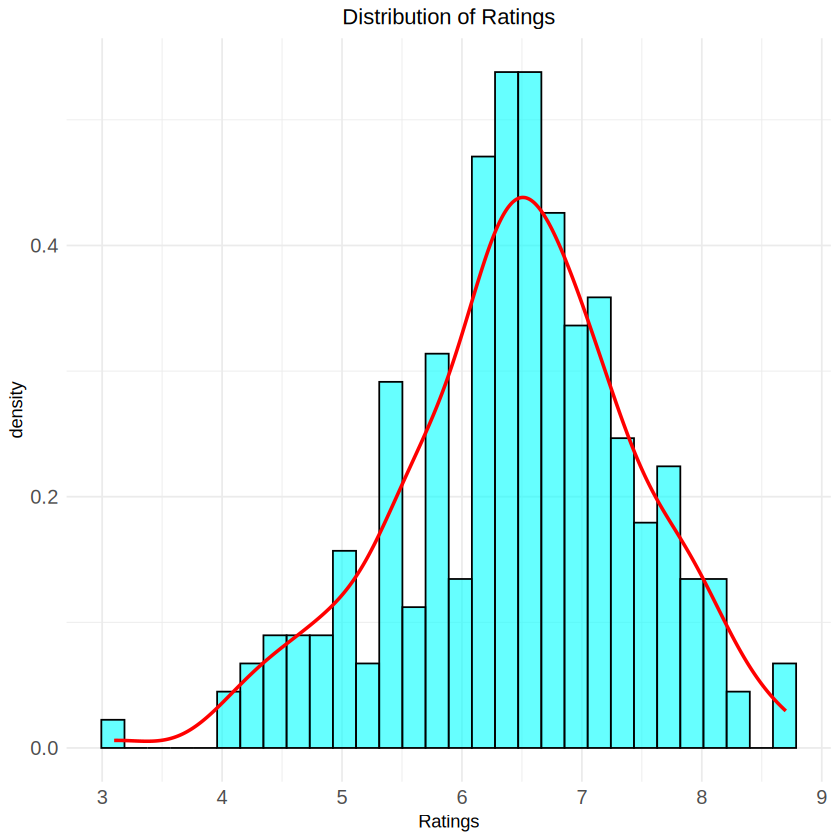
\includegraphics[width=0.75\columnwidth]{csm_figures/ratings_original_distribution.png}
    \caption{Phân phối ban đầu của Ratings.}
    \label{fig:ratings_original_distribution}
\end{figure}

Nhận xét:
\begin{itemize}
    \item Nhìn vào biểu đồ, ta thấy phân phối của biến Ratings tương đối xấp xỉ chuẩn.
\end{itemize}

Ta thử sử dụng log-transform nó và thu được phân phối như hình bên dưới.

\begin{figure}[H]
    \centering
    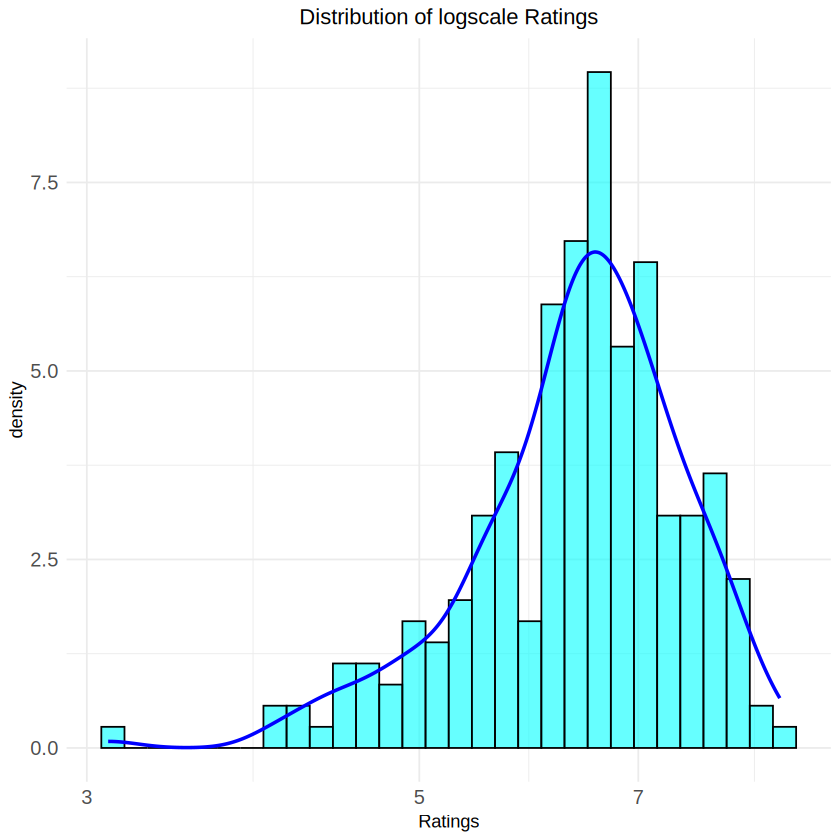
\includegraphics[width=0.75\columnwidth]{csm_figures/ratings_logscale_distribution.png}
    \caption{Phân phối sau khi log-scale của Ratings.}
    \label{fig:ratings_logscale_distribution}
\end{figure}
Nhận xét:
\begin{itemize}
    \item Ta nhận thấy sau khi sử dụng log-transform, dữ liệu bị lệch trái (lệch âm). Do đó, ta thử sử dụng biến đổi box-cox.
\end{itemize}

\begin{figure}[H]
    \centering
    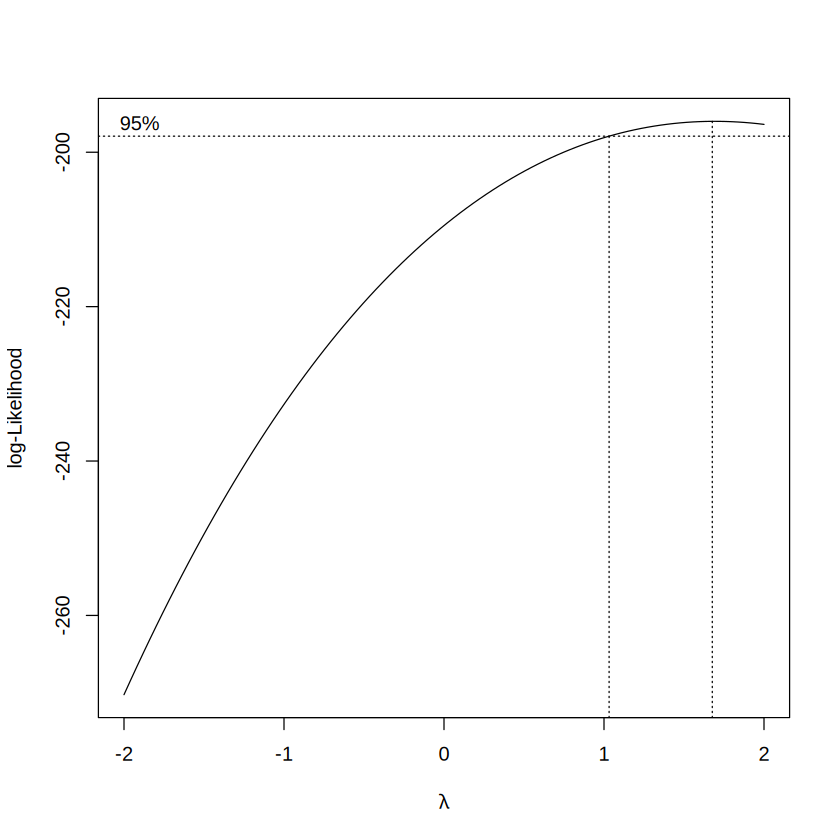
\includegraphics[width=0.75\columnwidth]{csm_figures/ratings_optimal_lambda.png}
    \caption{Log-likelihood với các giá trị $\lambda$ của Ratings.}
    \label{fig:ratings_optimal_lambda}
\end{figure}
Nhận xét:
\begin{itemize}
    \item Dựa trên biểu đồ, ta tìm được giá trị lambda tối ưu với mức ý nghĩa 5\% là 1.677.
\end{itemize}

Và ta thực hiện biến đổi dữ liệu với giá trị lambda vừa tìm được.
\begin{figure}[H]
    \centering
    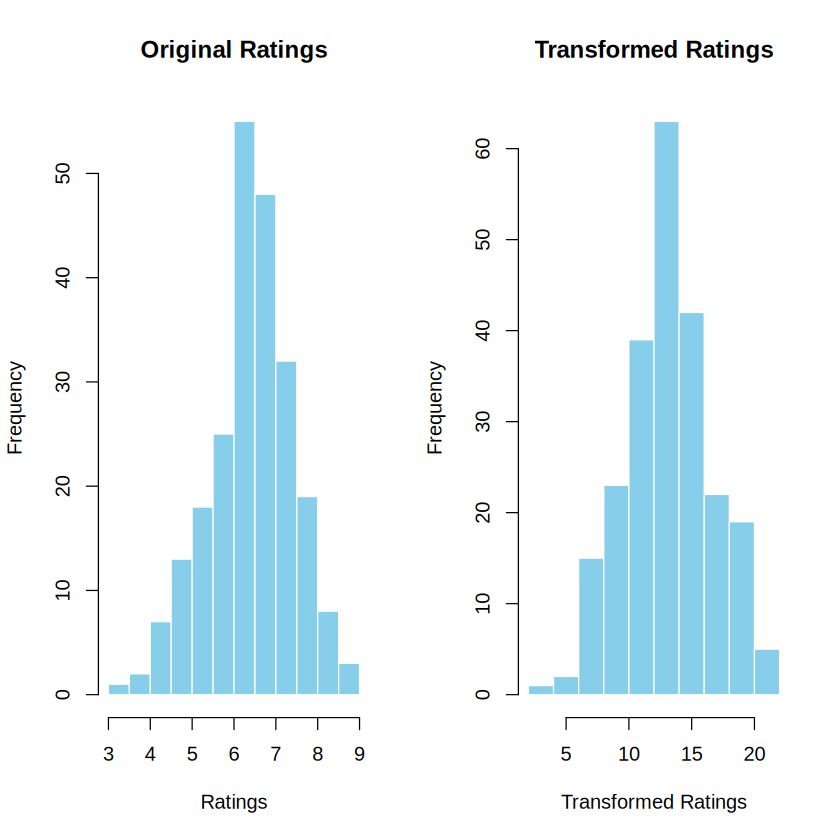
\includegraphics[width=0.75\columnwidth]{csm_figures/ratings_transformed_distribution.png}
    \caption{Phân phối trước và sau khi biến đổi của Gross.}
    \label{fig:ratings_transformed_distribution}
\end{figure}
Nhận xét:
\begin{itemize}
    \item Ta có được giá trị lambda tối ưu là 1.677 và sử dụng giá trị này để biến đổi biến Ratings. Biểu đồ histogram phía bên dưới thể hiện phân phối của biến này trước và sau khi biến đổi. Dễ dàng thấy được, sau khi biến đổi, biến này đã tương đối chuẩn hơn.
\end{itemize}

\subsubsection{Phân tích biến Budget}

Trong phần này, chúng ta sẽ xem xét biến Budget thể hiện chi phí đầu tư cho một bộ phim.

\begin{figure}[H]
    \centering
    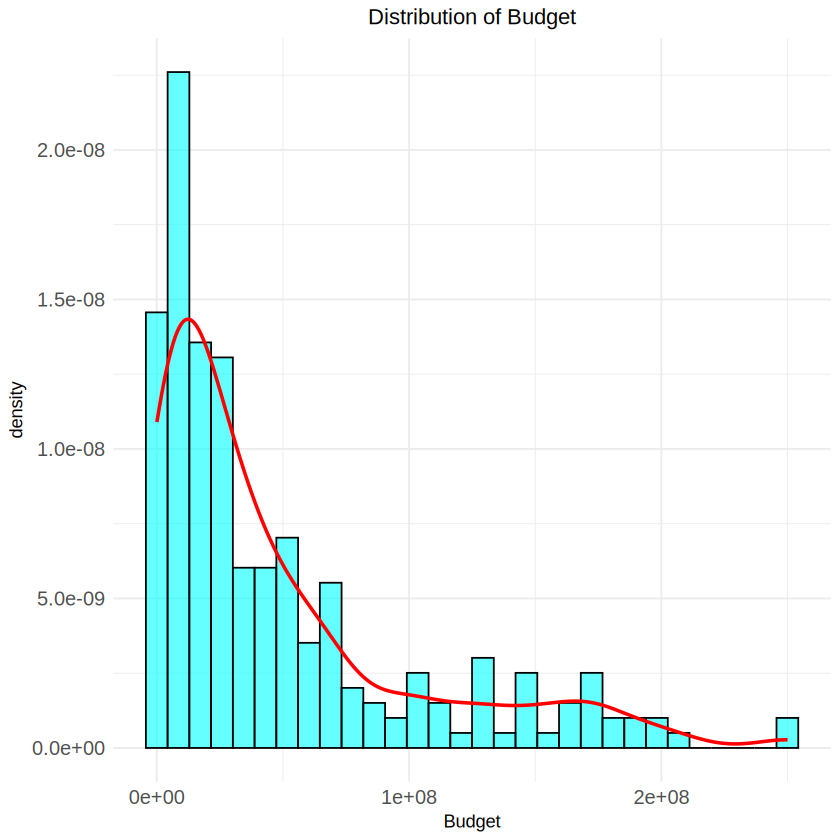
\includegraphics[width=0.75\columnwidth]{csm_figures/budget_original_distribution.png}
    \caption{Phân phối ban đầu của Budget.}
    \label{fig:budget_original_distribution}
\end{figure}

Nhận xét:
\begin{itemize}
    \item Nhìn vào biểu đồ, ta thấy phân phối của biến Ratings bị lệch phải (lệch dương).
\end{itemize}

Ta thử sử dụng log-transform nó và thu được phân phối như hình bên dưới.

\begin{figure}[H]
    \centering
    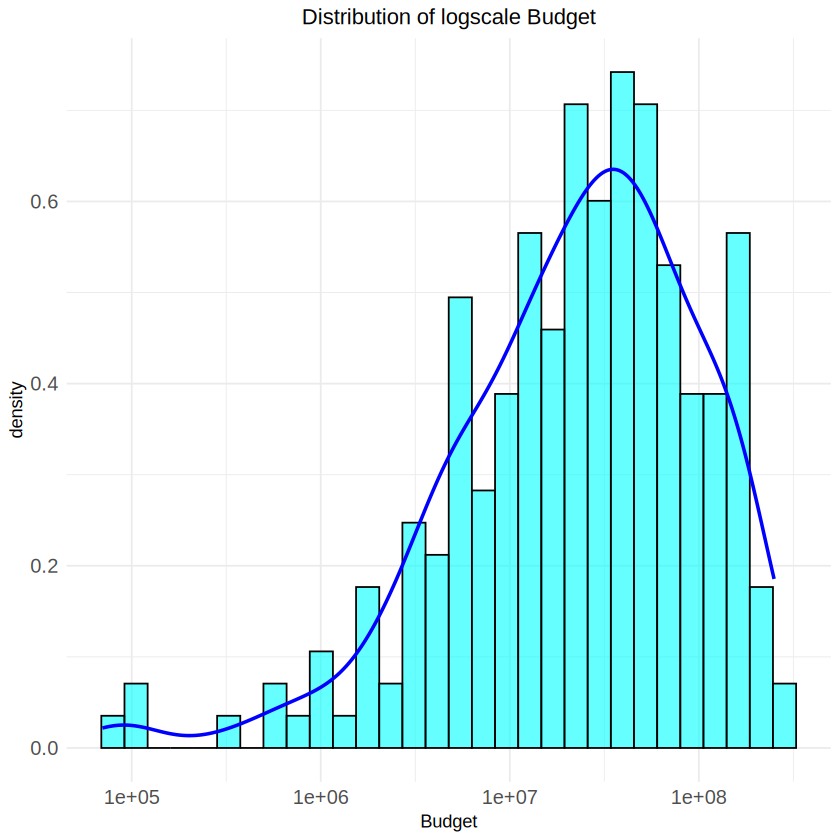
\includegraphics[width=0.75\columnwidth]{csm_figures/budget_logscale_distribution.png}
    \caption{Phân phối sau khi log-scale của Budget.}
    \label{fig:budget_logscale_distribution}
\end{figure}
Nhận xét:
\begin{itemize}
    \item Ta nhận thấy sau khi sử dụng log-transform, dữ liệu tương đối xấp xỉ chuẩn. Do đó, ta thử sử dụng biến đổi box-cox.
\end{itemize}

\begin{figure}[H]
    \centering
    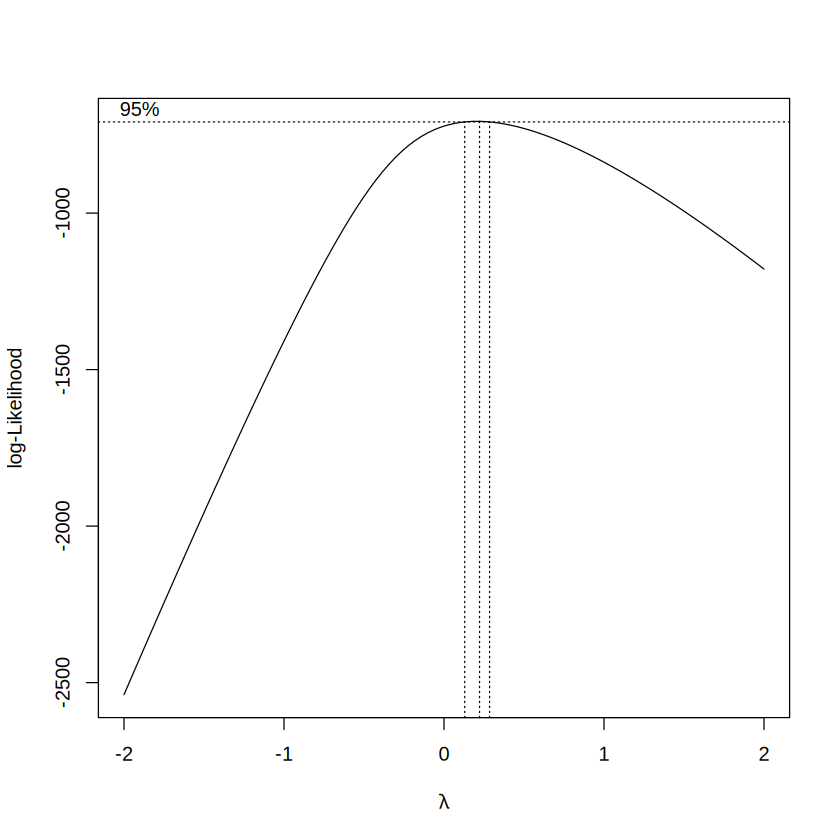
\includegraphics[width=0.75\columnwidth]{csm_figures/budget_optimal_lambda.png}
    \caption{Log-likelihood với các giá trị $\lambda$ của Budget.}
    \label{fig:budget_optimal_lambda}
\end{figure}
Nhận xét:
\begin{itemize}
    \item Dựa trên biểu đồ, ta tìm được giá trị lambda tối ưu với mức ý nghĩa 5\% là 0.222.
\end{itemize}

Và ta thực hiện biến đổi dữ liệu với giá trị lambda vừa tìm được.
\begin{figure}[H]
    \centering
    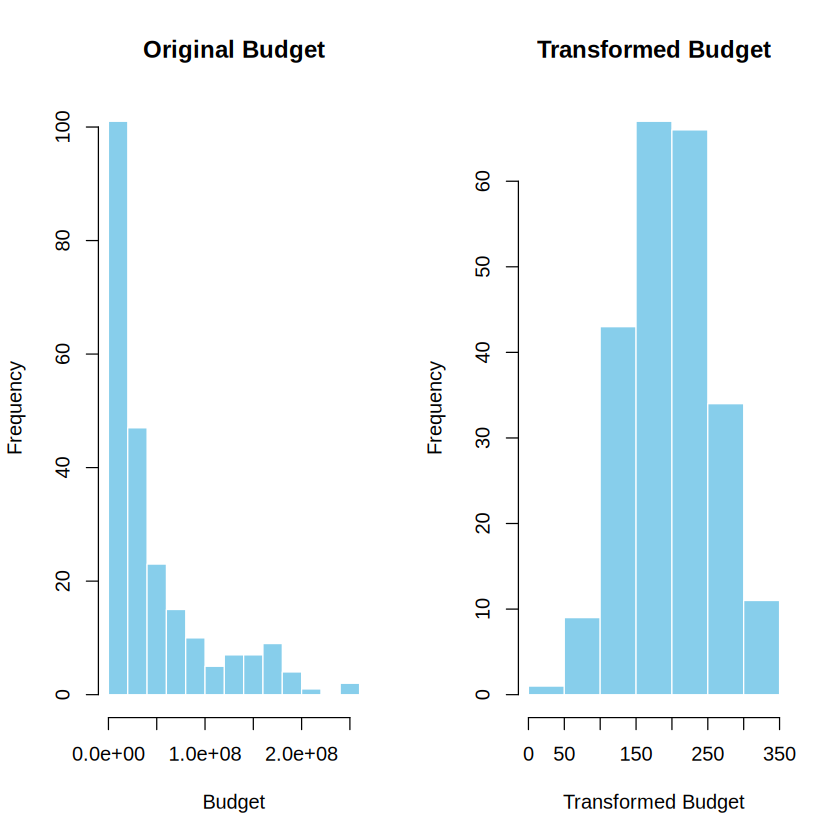
\includegraphics[width=0.75\columnwidth]{csm_figures/budget_transformed_distribution.png}
    \caption{Phân phối trước và sau khi biến đổi của Budget.}
    \label{fig:budget_transformed_distribution}
\end{figure}
Nhận xét:
\begin{itemize}
    \item Ta có được giá trị lambda tối ưu là 0.2222 và sử dụng giá trị này để biến đổi biến Budget. Biểu đồ histogram phía bên dưới thể hiện phân phối của biến này trước và sau khi biến đổi. Dễ dàng thấy được, sau khi biến đổi, biến này đã tương đối chuẩn hơn.
\end{itemize}

\subsubsection{Phân tích biến Screens}

Trong phần này, chúng ta sẽ xem xét biến Screens thể hiện số rạp chiếu của một bộ phim.

\begin{figure}[H]
    \centering
    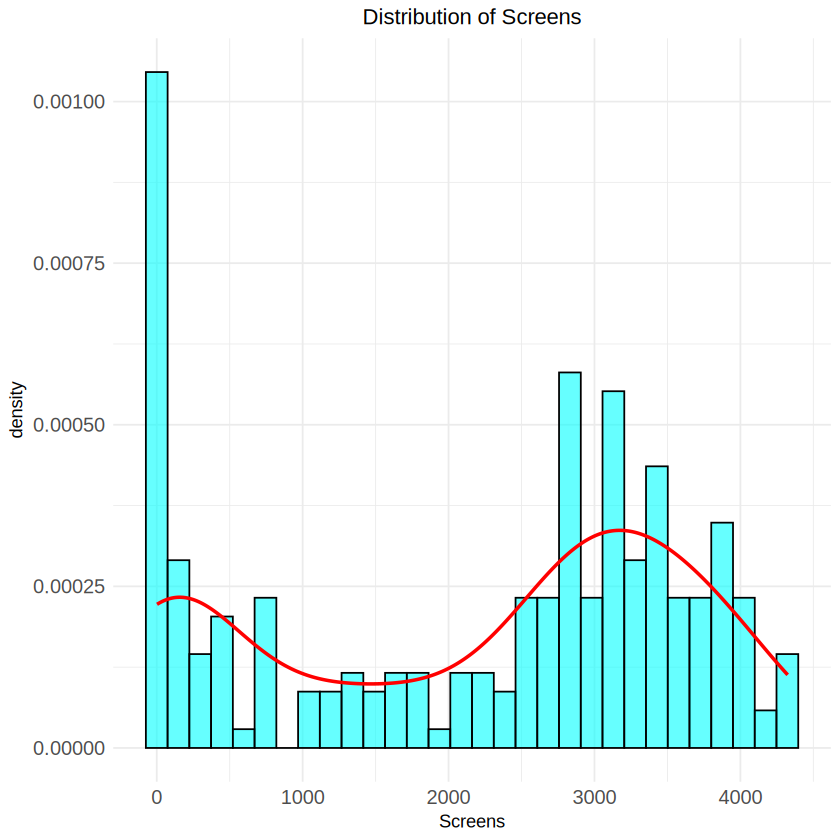
\includegraphics[width=0.75\columnwidth]{csm_figures/screens_original_distribution.png}
    \caption{Phân phối ban đầu của Screens.}
    \label{fig:screens_original_distribution}
\end{figure}

Nhận xét:
\begin{itemize}
    \item Nhìn vào biểu đồ, ta thấy phân phối của biến Screens có phân phối hai đỉnh, trong đó một đỉnh tập trung ở gần 0 và một đỉnh tập trung ở 3000.
\end{itemize}

Ta thử sử dụng log-transform nó và thu được phân phối như hình bên dưới.

\begin{figure}[H]
    \centering
    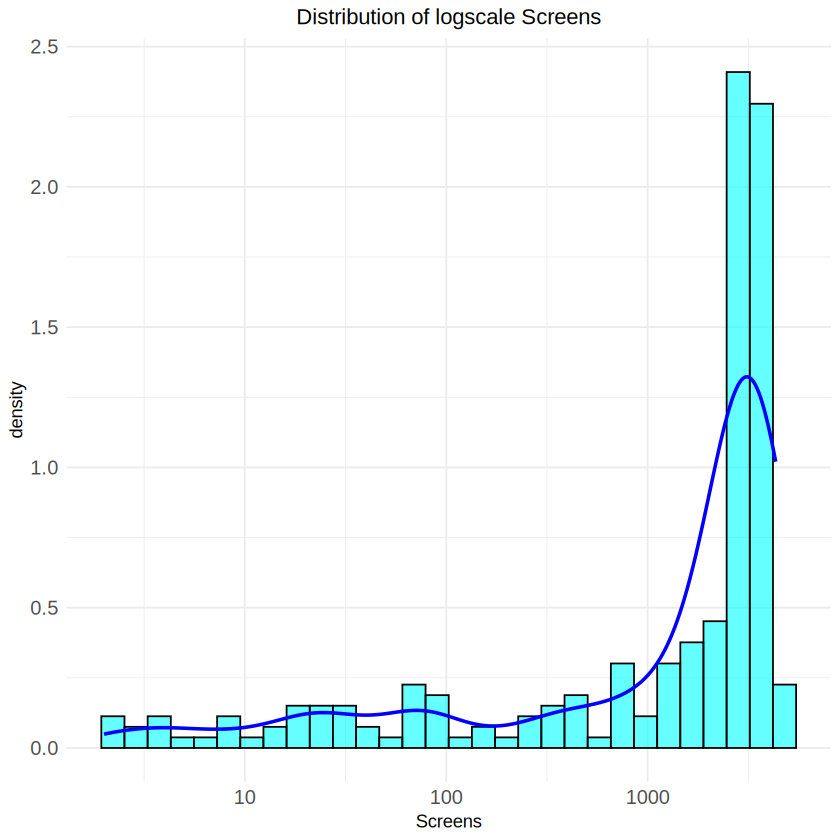
\includegraphics[width=0.75\columnwidth]{csm_figures/screens_logscale_distribution.png}
    \caption{Phân phối sau khi log-scale của Screens.}
    \label{fig:screens_logscale_distribution}
\end{figure}
Nhận xét:
\begin{itemize}
    \item Ta nhận thấy sau khi sử dụng log-transform, dữ liệu tương đối bị lệch phải (lệch dương). Do đó, ta thử sử dụng biến đổi box-cox.
\end{itemize}

\begin{figure}[H]
    \centering
    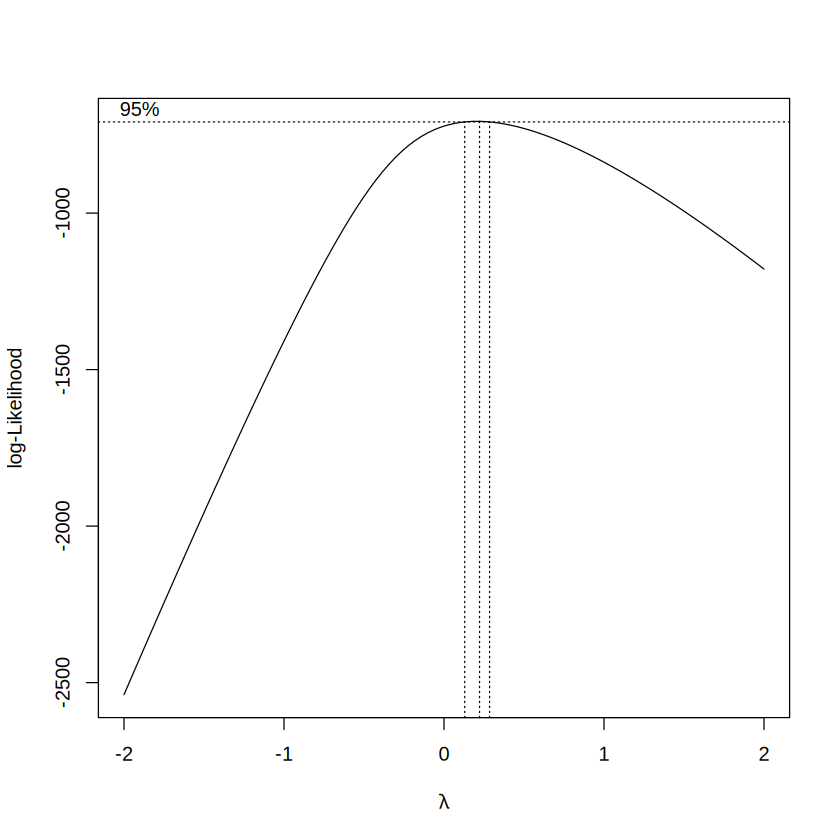
\includegraphics[width=0.75\columnwidth]{csm_figures/budget_optimal_lambda.png}
    \caption{Log-likelihood với các giá trị $\lambda$ của Screens.}
    \label{fig:screens_optimal_lambda}
\end{figure}
Nhận xét:
\begin{itemize}
    \item Dựa trên biểu đồ, ta tìm được giá trị lambda tối ưu với mức ý nghĩa 5\% là 0.5858.
\end{itemize}

Và ta thực hiện biến đổi dữ liệu với giá trị lambda vừa tìm được.
\begin{figure}[H]
    \centering
    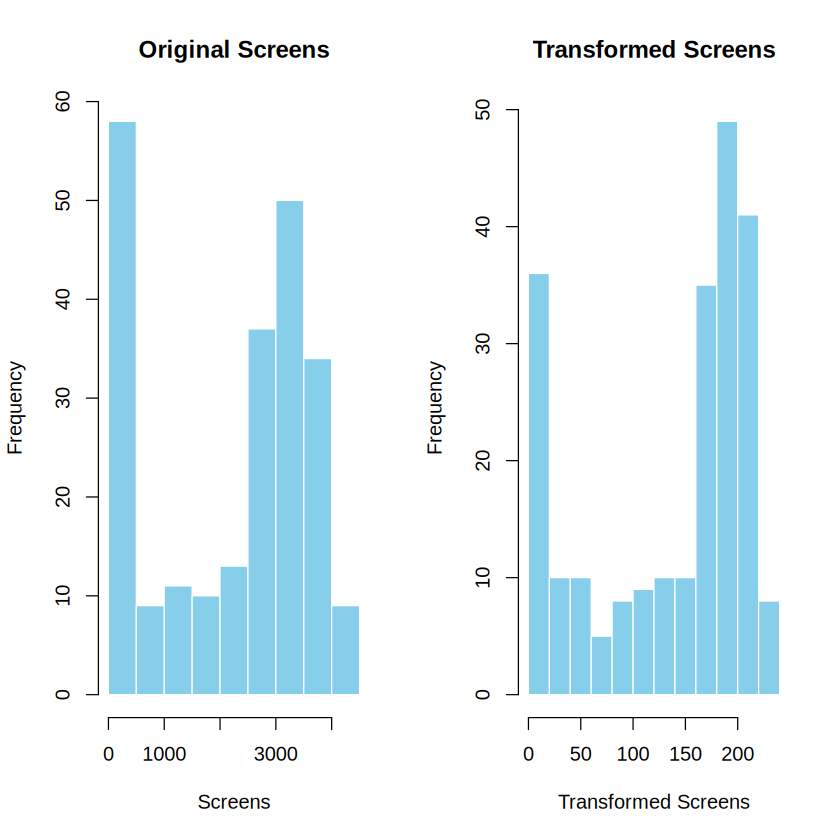
\includegraphics[width=0.75\columnwidth]{csm_figures/screens_transformed_distribution.png}
    \caption{Phân phối trước và sau khi biến đổi của Screens.}
    \label{fig:screens_transformed_distribution}
\end{figure}
Nhận xét:
\begin{itemize}
    \item Ta có được giá trị lambda tối ưu là 0.2222 và sử dụng giá trị này để biến đổi biến Screens. Biểu đồ histogram phía bên dưới thể hiện phân phối của biến này trước và sau khi biến đổi. Dễ dàng thấy được, sau khi biến đổi, biến này vẫn có phân phối hai đỉnh trong đó một đỉnh tập trung ở gần 0 còn đỉnh còn lại tập trung ở 200.
    \item Như vậy, có thể có ngoại lai xuất hiện, ta cần thực hiện loại bỏ các cực ngoại lai để tiếp tục xây dựng môn hình.
\end{itemize}

\subsubsection{Phân tích biến Sequel}

Trong phần này, chúng ta sẽ xem xét biến Sequel thể hiện các phần của một bộ phim.

\begin{figure}[H]
    \centering
    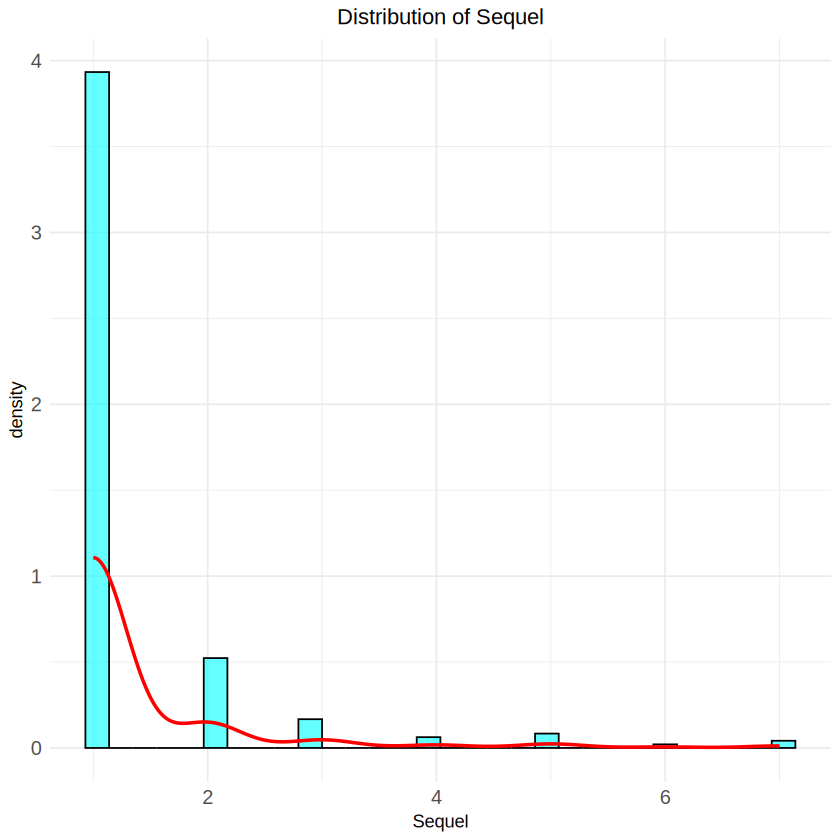
\includegraphics[width=0.75\columnwidth]{csm_figures/sequel_original_distribution.png}
    \caption{Phân phối ban đầu của Sequel.}
    \label{fig:sequel_original_distribution}
\end{figure}

Nhận xét:
\begin{itemize}
    \item Nhìn vào biểu đồ, ta thấy phân phối của biến Ratings bị lệch trái (lệch âm).
    \item Đa số các bộ phim chỉ có một phần phim
    \item Rất ít các bộ phim có từ 4 phần trở lên
    \item Số lượng các bộ phim có 5 phần nhiều hơn các bộ phim có 4 phần, và 6 phần
\end{itemize}

\subsubsection{Phân tích biến Sentiment}

Trong phần này, chúng ta sẽ xem xét biến Sentiment thể hiện ý kiến khán giả đối với một bộ phim.

\begin{figure}[H]
    \centering
    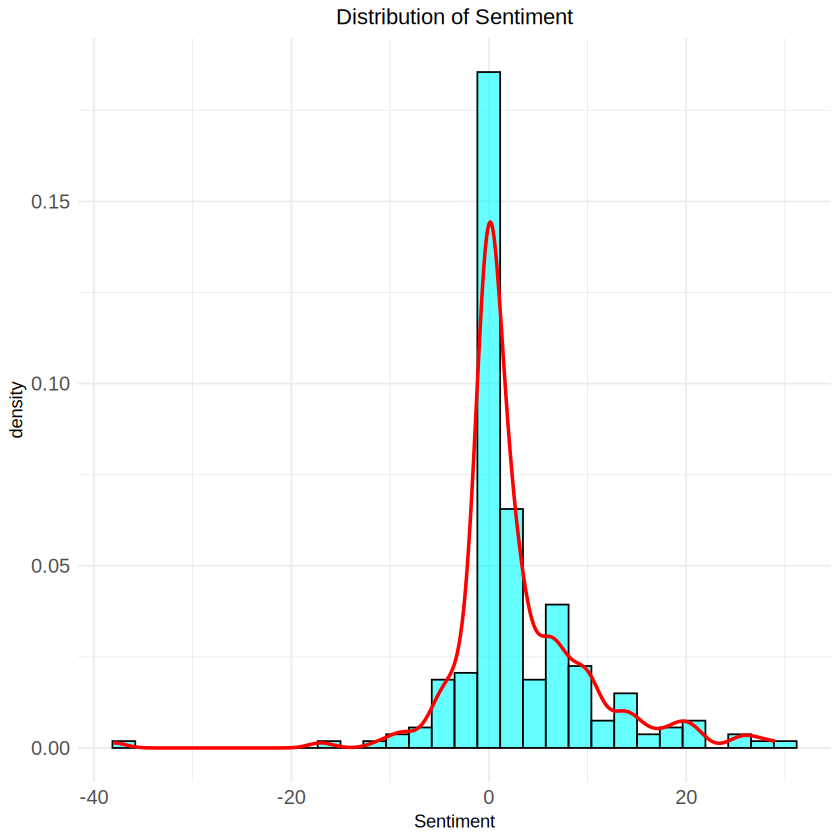
\includegraphics[width=0.75\columnwidth]{csm_figures/sentiment_original_distribution.png}
    \caption{Phân phối ban đầu của Sentiment.}
    \label{fig:sentiment_original_distribution}
\end{figure}

Nhận xét:
\begin{itemize}
    \item Nhìn vào biểu đồ, ta thấy phân phối của biến Sentiment có phân phối xấp xỉ chuẩn.
    \item Tuy nhiên, các giá trị tập trung ở 0 rất cao.
\end{itemize}

Ta thử sử dụng log-transform nó và thu được phân phối như hình bên dưới.

\begin{figure}[H]
    \centering
    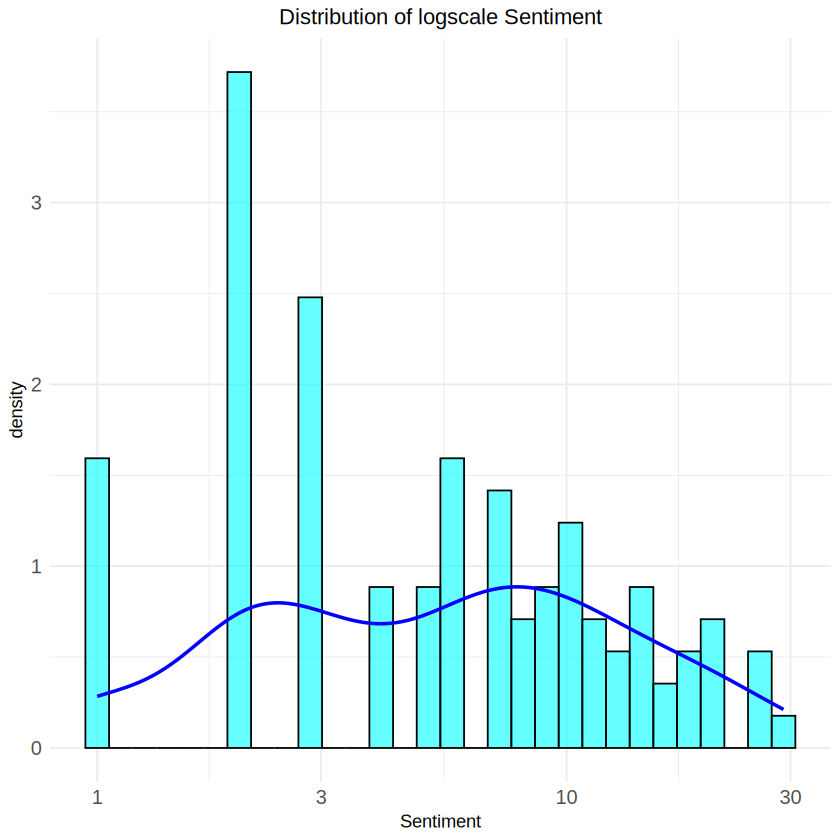
\includegraphics[width=0.75\columnwidth]{csm_figures/sentiment_logscale_distribution.png}
    \caption{Phân phối sau khi log-scale của Sentiment.}
    \label{fig:sentiment_logscale_distribution}
\end{figure}
Nhận xét:
\begin{itemize}
    \item Ta nhận thấy sau khi sử dụng log-transform, dữ liệu tương đối lệch trái (lệch dương). Do đó, ta thử sử dụng biến đổi box-cox.
\end{itemize}

\begin{figure}[H]
    \centering
    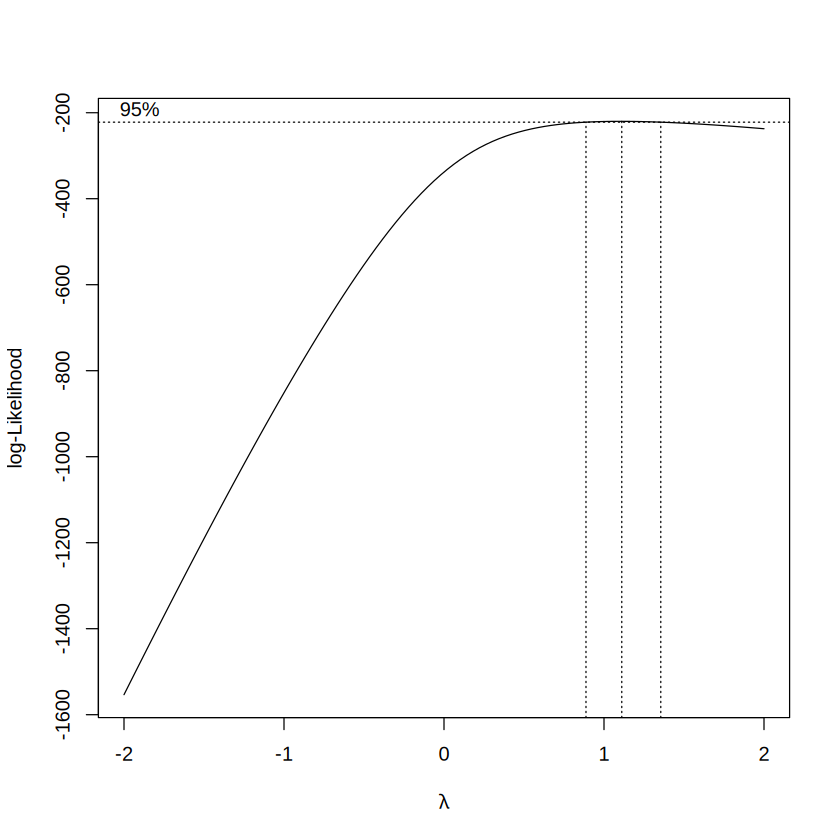
\includegraphics[width=0.75\columnwidth]{csm_figures/sentiment_optimal_lambda.png}
    \caption{Log-likelihood với các giá trị $\lambda$ của Sentiment.}
    \label{fig:sentiment_optimal_lambda}
\end{figure}
Nhận xét:
\begin{itemize}
    \item Dựa trên biểu đồ, ta tìm được giá trị lambda tối ưu với mức ý nghĩa 5\% là 1.111.
\end{itemize}

Và ta thực hiện biến đổi dữ liệu với giá trị lambda vừa tìm được.
\begin{figure}[H]
    \centering
    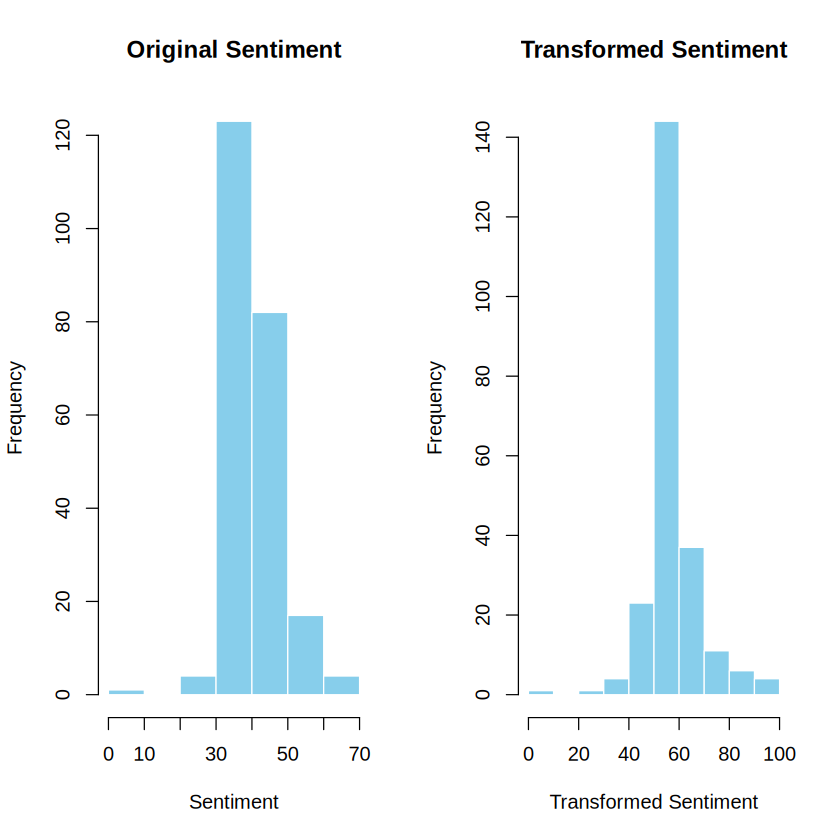
\includegraphics[width=0.75\columnwidth]{csm_figures/sentiment_transformed_distribution.png}
    \caption{Phân phối trước và sau khi biến đổi của Sentiment.}
    \label{fig:sentiment_transformed_distribution}
\end{figure}
Nhận xét:
\begin{itemize}
    \item Ta có được giá trị lambda tối ưu là 1.11 và sử dụng giá trị này để biến đổi biến Sentiment. Biểu đồ histogram phía bên dưới thể hiện phân phối của biến này trước và sau khi biến đổi. Dễ dàng thấy được, sau khi biến đổi, biến này đã tương đối chuẩn hơn.
\end{itemize}

\subsubsection{Phân tích biến Views}

Trong phần này, chúng ta sẽ xem xét biến Views thể hiện số lượt xem của một bộ phim.

\begin{figure}[H]
    \centering
    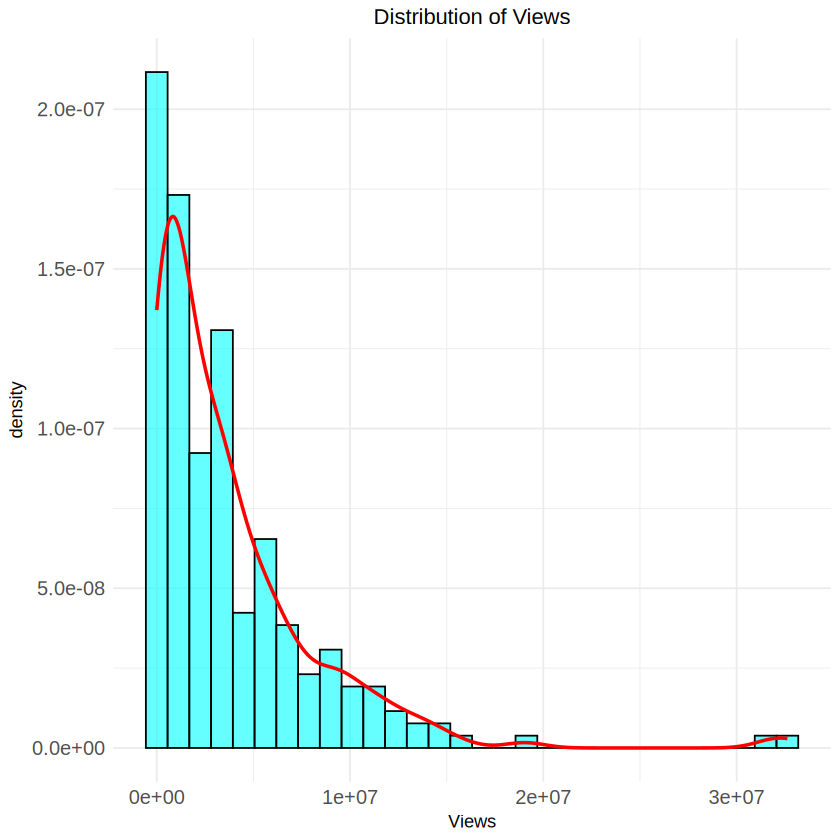
\includegraphics[width=0.75\columnwidth]{csm_figures/views_original_distribution.png}
    \caption{Phân phối ban đầu của Views.}
    \label{fig:views_original_distribution}
\end{figure}

Nhận xét:
\begin{itemize}
    \item Nhìn vào biểu đồ, ta thấy phân phối của biến Views có phân phối bị lệch trái (lệch dương).
\end{itemize}

Ta thử sử dụng log-transform nó và thu được phân phối như hình bên dưới.

\begin{figure}[H]
    \centering
    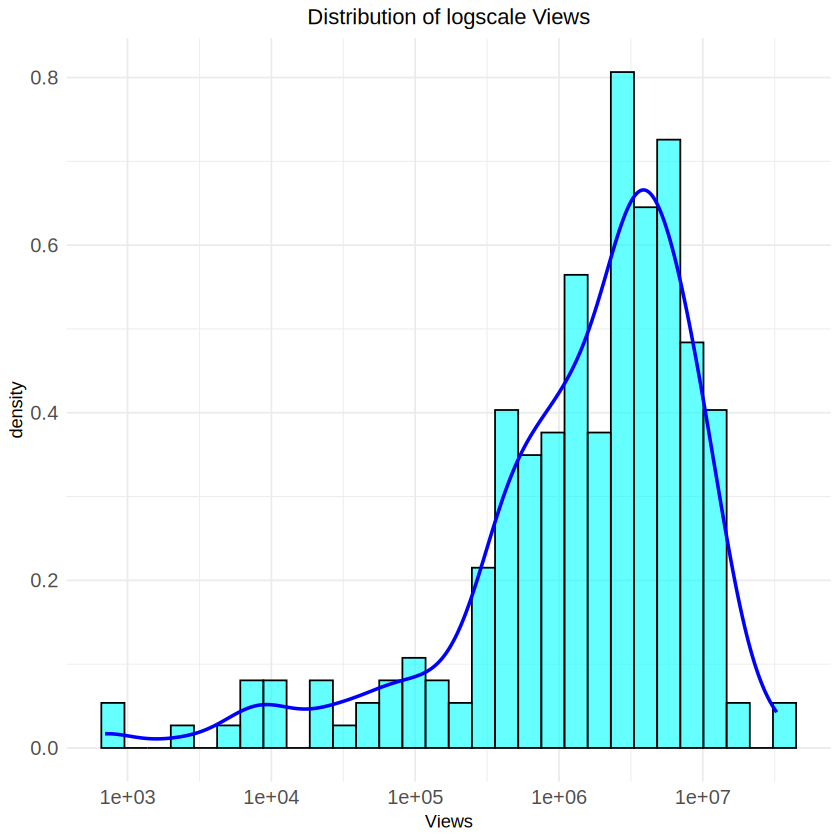
\includegraphics[width=0.75\columnwidth]{csm_figures/views_logscale_distribution.png}
    \caption{Phân phối sau khi log-scale của Views.}
    \label{fig:views_logscale_distribution}
\end{figure}
Nhận xét:
\begin{itemize}
    \item Ta nhận thấy sau khi sử dụng log-transform, dữ liệu tương đối lệch phải (lệch âm). Do đó, ta thử sử dụng biến đổi box-cox.
\end{itemize}

\begin{figure}[H]
    \centering
    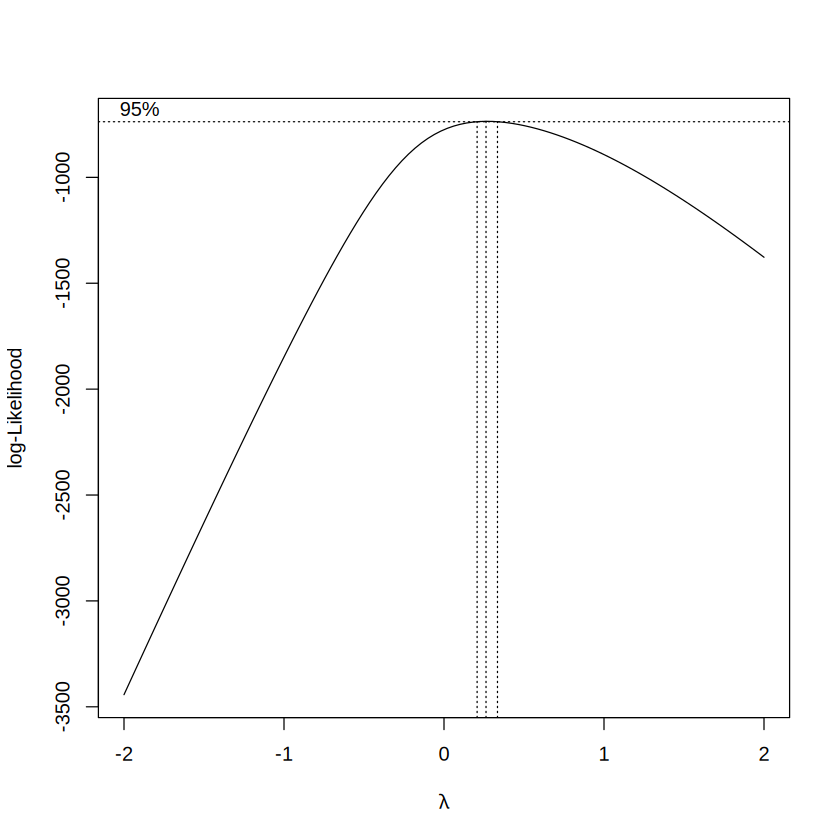
\includegraphics[width=0.75\columnwidth]{csm_figures/views_optimal_lambda.png}
    \caption{Log-likelihood với các giá trị $\lambda$ của Views.}
    \label{fig:views_optimal_lambda}
\end{figure}
Nhận xét:
\begin{itemize}
    \item Dựa trên biểu đồ, ta tìm được giá trị lambda tối ưu với mức ý nghĩa 5\% là 0.2626.
\end{itemize}

Và ta thực hiện biến đổi dữ liệu với giá trị lambda vừa tìm được.
\begin{figure}[H]
    \centering
    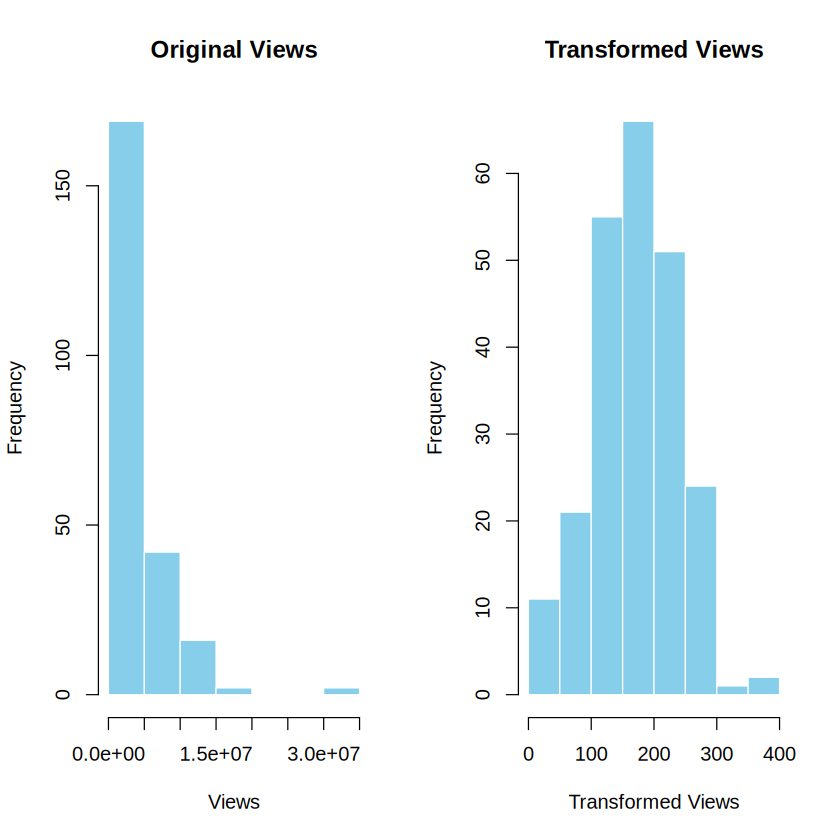
\includegraphics[width=0.75\columnwidth]{csm_figures/views_transformed_distribution.png}
    \caption{Phân phối trước và sau khi biến đổi của Views.}
    \label{fig:views_transformed_distribution}
\end{figure}
Nhận xét:
\begin{itemize}
    \item Ta có được giá trị lambda tối ưu là 0.2626 và sử dụng giá trị này để biến đổi biến Views. Biểu đồ histogram phía bên dưới thể hiện phân phối của biến này trước và sau khi biến đổi. Dễ dàng thấy được, sau khi biến đổi, biến này đã tương đối chuẩn hơn.
\end{itemize}

\subsubsection{Phân tích biến Likes}

Trong phần này, chúng ta sẽ xem xét biến Likes thể hiện số lượt thích của một bộ phim.

\begin{figure}[H]
    \centering
    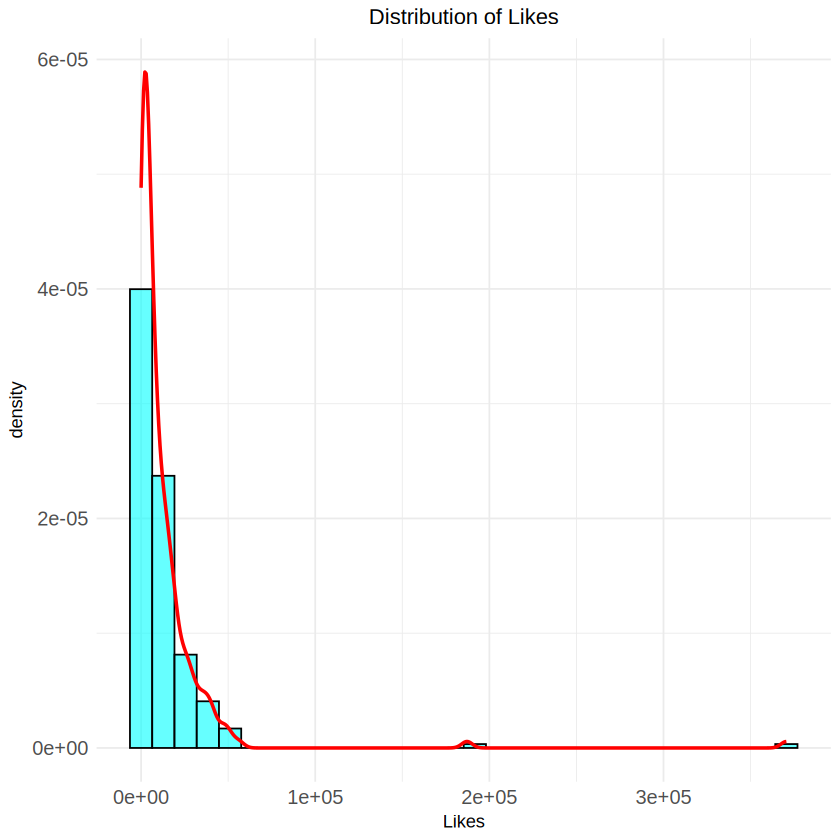
\includegraphics[width=0.75\columnwidth]{csm_figures/likes_original_distribution.png}
    \caption{Phân phối ban đầu của Likes.}
    \label{fig:likes_original_distribution}
\end{figure}

Nhận xét:
\begin{itemize}
    \item Nhìn vào biểu đồ, ta thấy phân phối của biến Likes có phân phối bị lệch trái (lệch dương).
\end{itemize}

Ta thử sử dụng log-transform nó và thu được phân phối như hình bên dưới.

\begin{figure}[H]
    \centering
    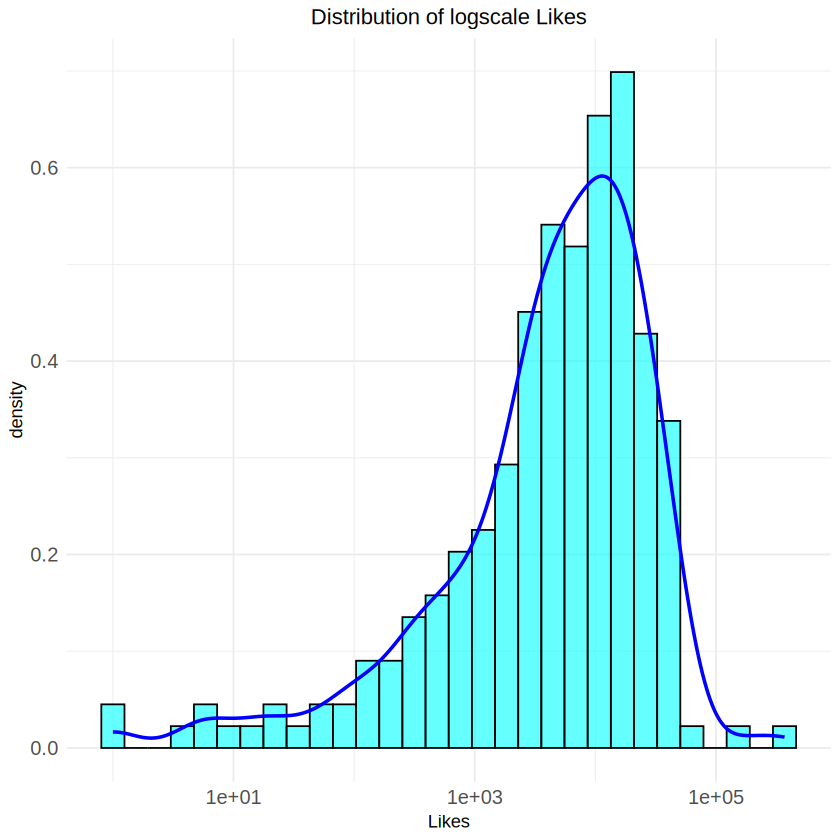
\includegraphics[width=0.75\columnwidth]{csm_figures/likes_logscale_distribution.png}
    \caption{Phân phối sau khi log-scale của Likes.}
    \label{fig:likes_logscale_distribution}
\end{figure}
Nhận xét:
\begin{itemize}
    \item Ta nhận thấy sau khi sử dụng log-transform, dữ liệu tương đối lệch phải (lệch âm). Do đó, ta thử sử dụng biến đổi box-cox.
\end{itemize}

\begin{figure}[H]
    \centering
    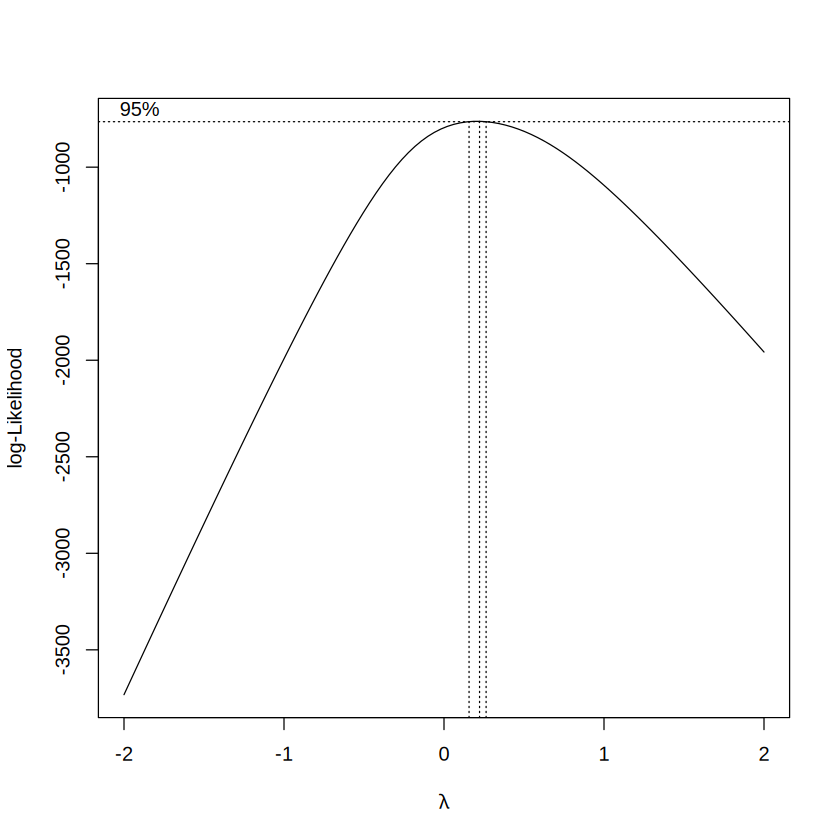
\includegraphics[width=0.75\columnwidth]{csm_figures/likes_optimal_lambda.png}
    \caption{Log-likelihood với các giá trị $\lambda$ của Likes.}
    \label{fig:likes_optimal_lambda}
\end{figure}
Nhận xét:
\begin{itemize}
    \item Dựa trên biểu đồ, ta tìm được giá trị lambda tối ưu với mức ý nghĩa 5\% là 0.2222.
\end{itemize}

Và ta thực hiện biến đổi dữ liệu với giá trị lambda vừa tìm được.
\begin{figure}[H]
    \centering
    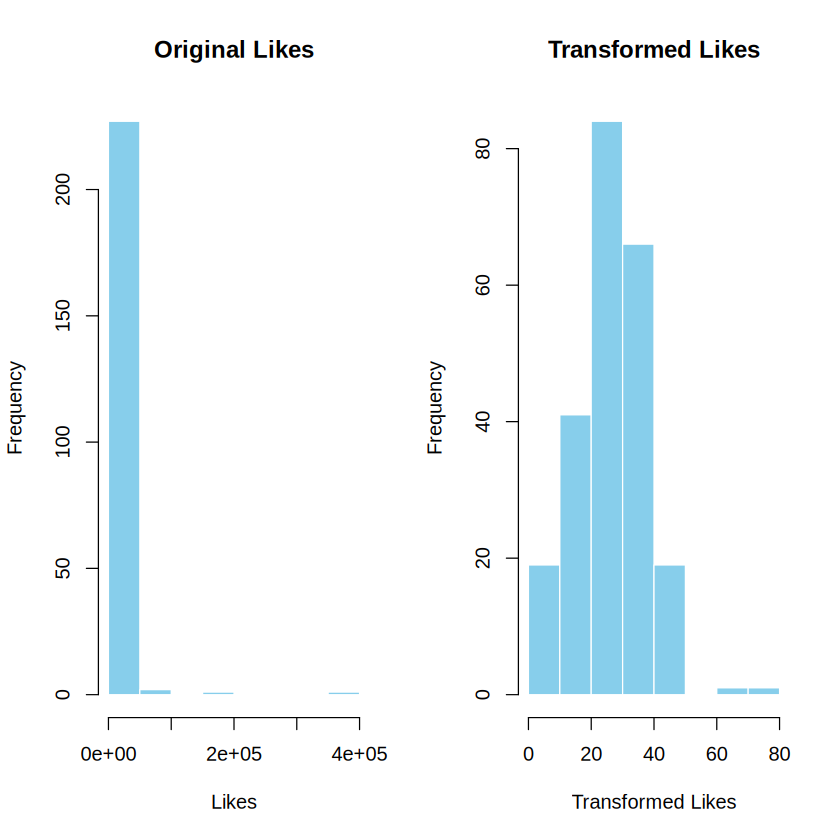
\includegraphics[width=0.75\columnwidth]{csm_figures/likes_transformed_distribution.png}
    \caption{Phân phối trước và sau khi biến đổi của Likes.}
    \label{fig:likes_transformed_distribution}
\end{figure}
Nhận xét:
\begin{itemize}
    \item Ta có được giá trị lambda tối ưu là 0.2222 và sử dụng giá trị này để biến đổi biến Likes. Biểu đồ histogram phía bên dưới thể hiện phân phối của biến này trước và sau khi biến đổi. Dễ dàng thấy được, sau khi biến đổi, biến này đã tương đối chuẩn hơn.
\end{itemize}

\subsubsection{Phân tích biến Comments}

Trong phần này, chúng ta sẽ xem xét biến Comments thể hiện số bình luận của một bộ phim.

\begin{figure}[H]
    \centering
    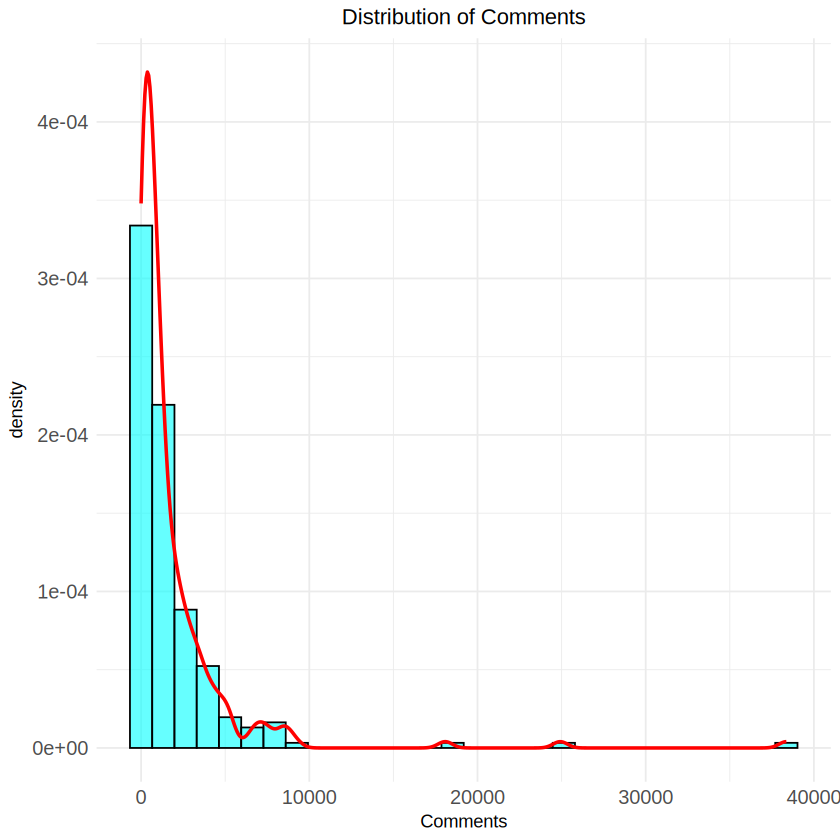
\includegraphics[width=0.75\columnwidth]{csm_figures/comments_original_distribution.png}
    \caption{Phân phối ban đầu của Likes.}
    \label{fig:comments_original_distribution}
\end{figure}

Nhận xét:
\begin{itemize}
    \item Nhìn vào biểu đồ, ta thấy phân phối của biến Comments có phân phối bị lệch trái (lệch dương).
\end{itemize}

Ta thử sử dụng log-transform nó và thu được phân phối như hình bên dưới.

\begin{figure}[H]
    \centering
    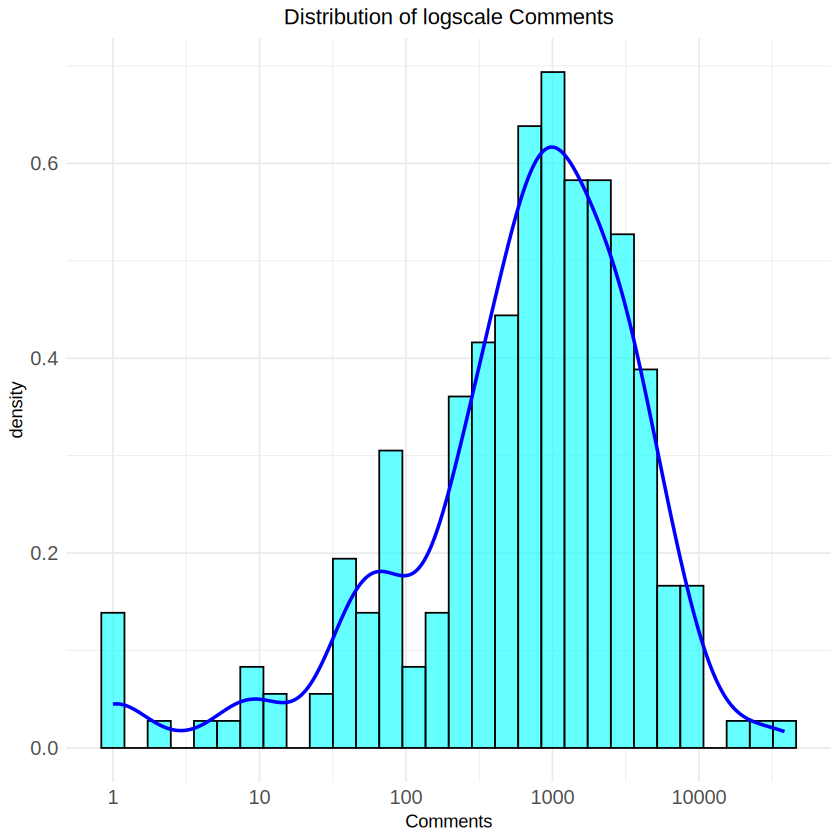
\includegraphics[width=0.75\columnwidth]{csm_figures/comments_logscale_distribution.png}
    \caption{Phân phối sau khi log-scale của Comments.}
    \label{fig:comments_logscale_distribution}
\end{figure}
Nhận xét:
\begin{itemize}
    \item Ta nhận thấy sau khi sử dụng log-transform, dữ liệu tương đối lệch phải (lệch âm). Do đó, ta thử sử dụng biến đổi box-cox.
\end{itemize}

\begin{figure}[H]
    \centering
    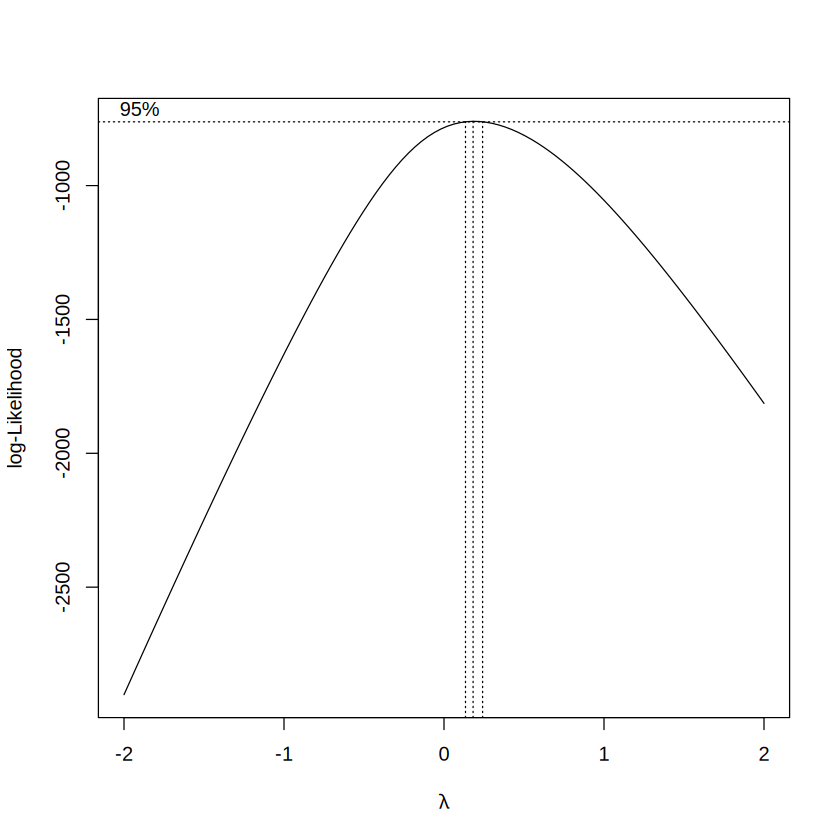
\includegraphics[width=0.75\columnwidth]{csm_figures/comments_optimal_lambda.png}
    \caption{Log-likelihood với các giá trị $\lambda$ của Comments.}
    \label{fig:comments_optimal_lambda}
\end{figure}
Nhận xét:
\begin{itemize}
    \item Dựa trên biểu đồ, ta tìm được giá trị lambda tối ưu với mức ý nghĩa 5\% là  0.1818.
\end{itemize}

Và ta thực hiện biến đổi dữ liệu với giá trị lambda vừa tìm được.
\begin{figure}[H]
    \centering
    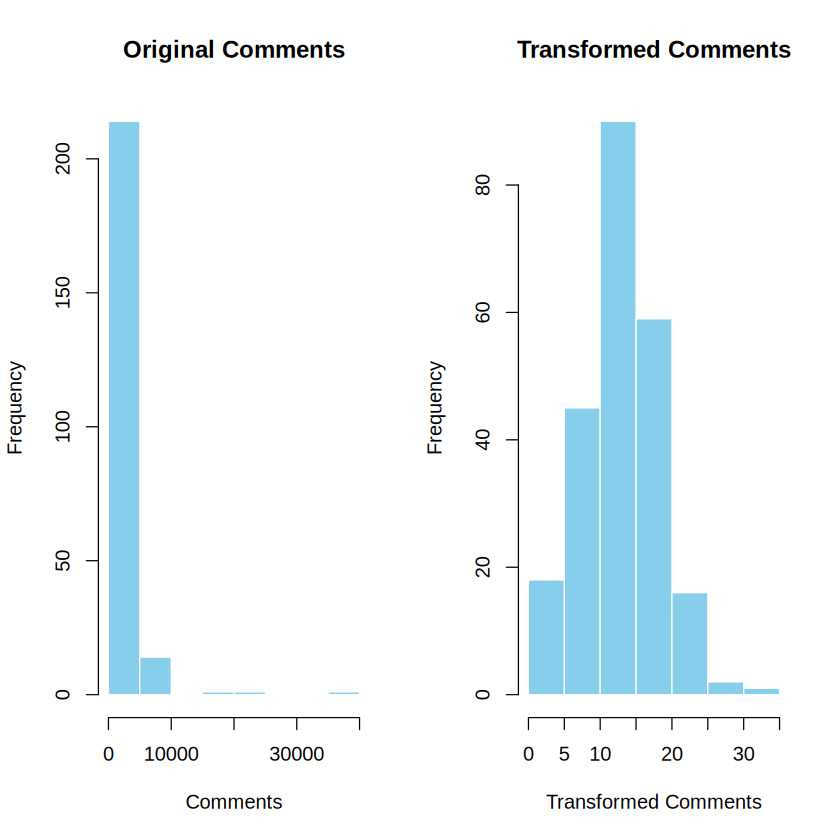
\includegraphics[width=0.75\columnwidth]{csm_figures/comments_transformed_distribution.png}
    \caption{Phân phối trước và sau khi biến đổi của Comments.}
    \label{fig:comments_transformed_distribution}
\end{figure}
Nhận xét:
\begin{itemize}
    \item Ta có được giá trị lambda tối ưu là  0.1818 và sử dụng giá trị này để biến đổi biến Comments. Biểu đồ histogram phía bên dưới thể hiện phân phối của biến này trước và sau khi biến đổi. Dễ dàng thấy được, sau khi biến đổi, biến này đã tương đối chuẩn hơn.
\end{itemize}

\subsubsection{Phân tích biến Gross}

\begin{figure}[H]
    \centering
    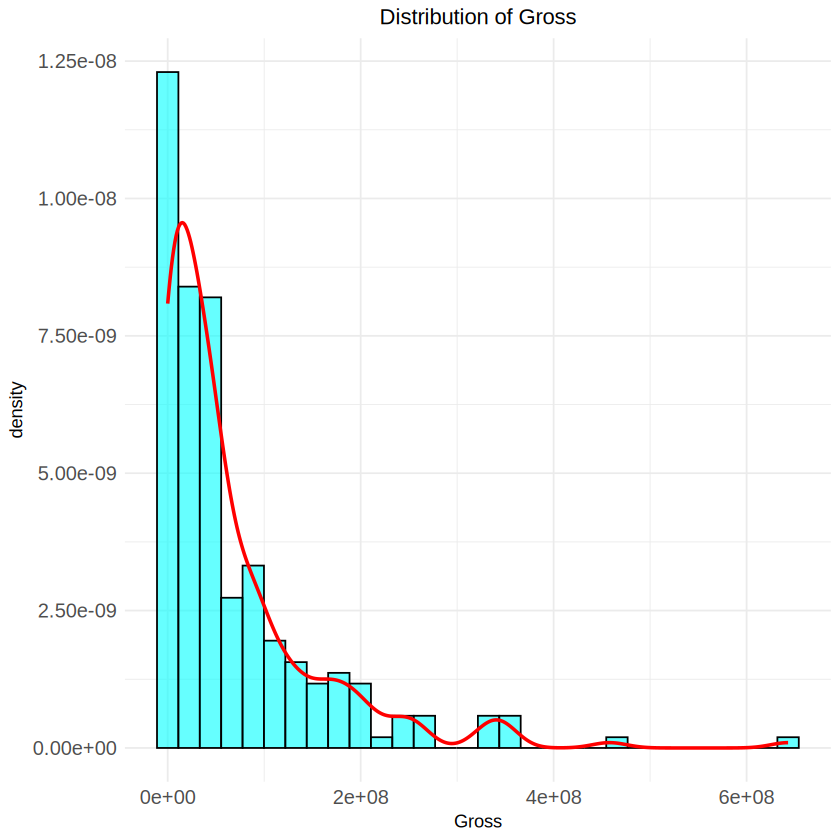
\includegraphics[width=0.75\columnwidth]{csm_figures/gross_original_distribution.png}
    \caption{Phân phối ban đầu của Gross.}
    \label{fig:gross_original_distribution}
\end{figure}

Nhận xét:
\begin{itemize}
    \item Nhìn vào biểu đồ, ta thấy phân phối của biến Gross bị lệch trái.
\end{itemize}

Ta thử sử dụng log-transform nó.

\begin{figure}[H]
    \centering
    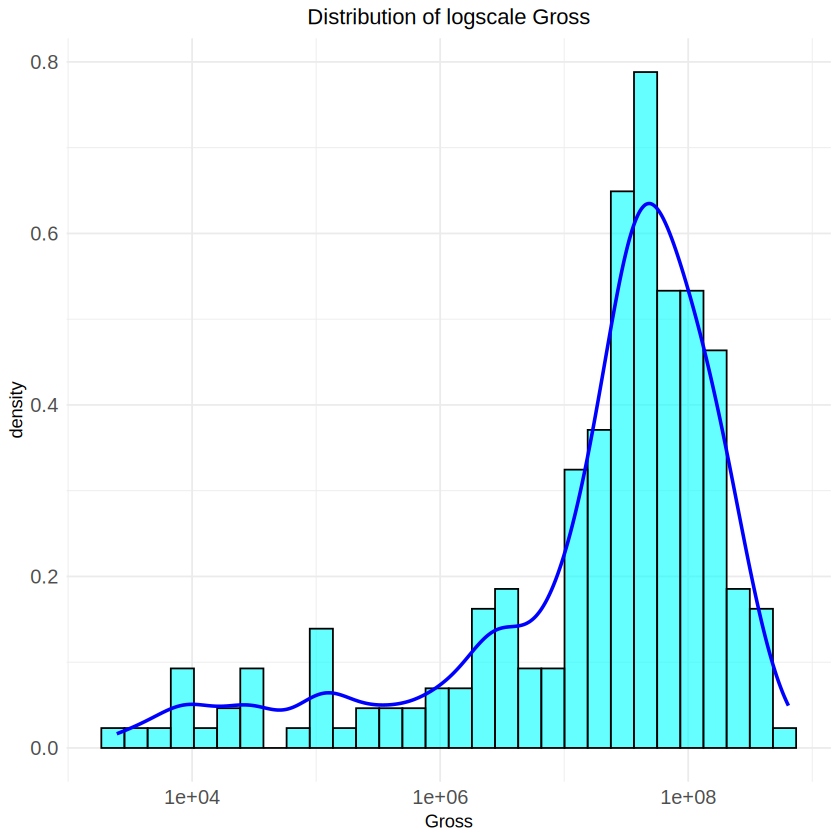
\includegraphics[width=0.75\columnwidth]{csm_figures/gross_logscale_distribution.png}
    \caption{Phân phối sau khi log-scale của Gross.}
    \label{fig:gross_logscale_distribution}
\end{figure}
Nhận xét:
\begin{itemize}
    \item Ta nhận thấy sau khi sử dụng log-transform, dữ liệu bị lệch phải. Do đó, ta thử sử dụng box-cox.
\end{itemize}

\begin{figure}[H]
    \centering
    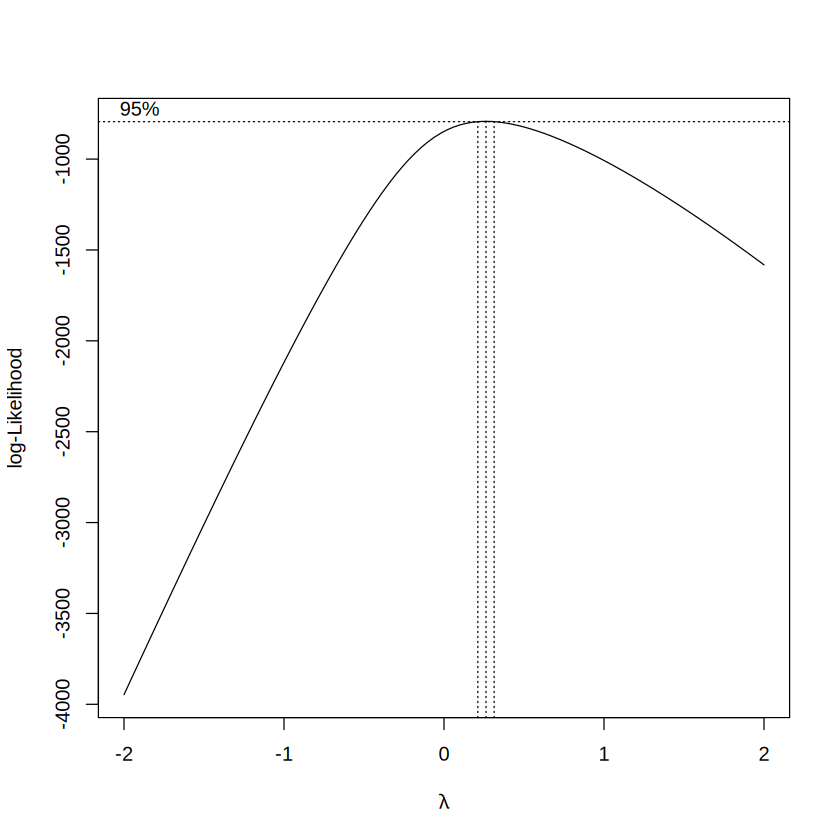
\includegraphics[width=0.75\columnwidth]{csm_figures/gross_optimal_lambda.png}
    \caption{Log-likelihood với các giá trị $\lambda$ của Gross.}
    \label{fig:gross_optimal_lambda}
\end{figure}
Nhận xét:
\begin{itemize}
    \item Dựa trên biểu đồ, ta tìm được giá trị lambda tối ưu với mức ý nghĩa 5\% là 0.262
\end{itemize}

Và ta thực hiện biến đổi dữ liệu với giá trị lambda vừa tìm được.
\begin{figure}[H]
    \centering
    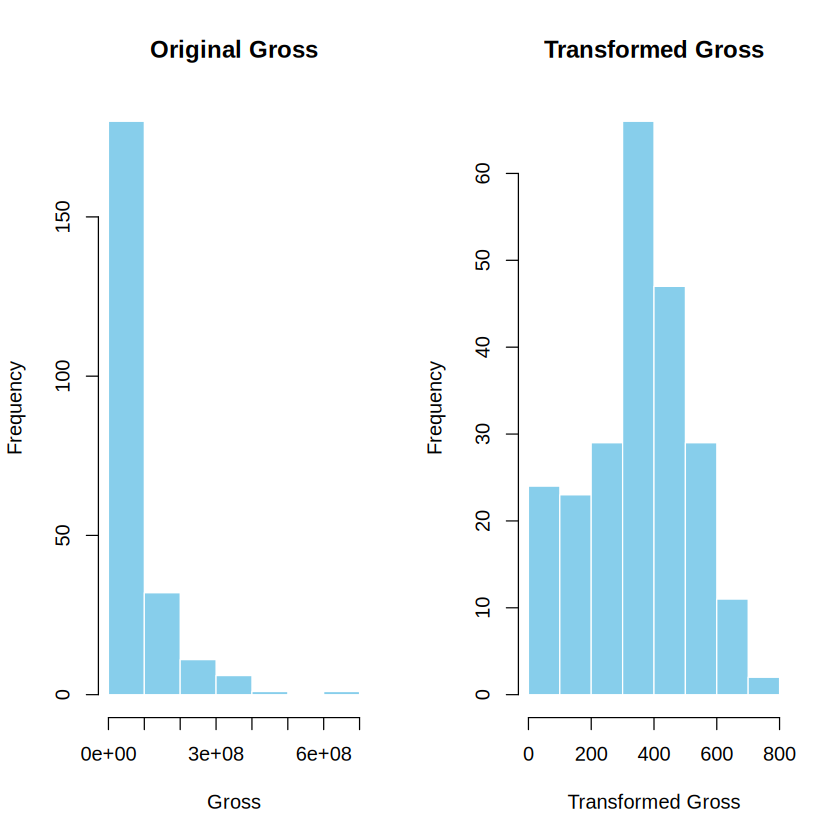
\includegraphics[width=0.75\columnwidth]{csm_figures/gross_transformed_distribution.png}
    \caption{Phân phối trước và sau khi biến đổi của Gross.}
    \label{fig:gross_transformed_distribution}
\end{figure}
Nhận xét:
\begin{itemize}
    \item Ta có được giá trị lambda tối ưu là 0.262 và sử dụng giá trị này để biến đổi biến Gross. Biểu đồ histogram phía bên dưới thể hiện phân phối của biến này trước và sau khi biến đổi. Dễ dàng thấy được, sau khi biến đổi, biến này đã tương đối chuẩn hơn.
\end{itemize}

\subsubsection{Phân tích biến AggregateFollowers}

\begin{figure}[H]
    \centering
    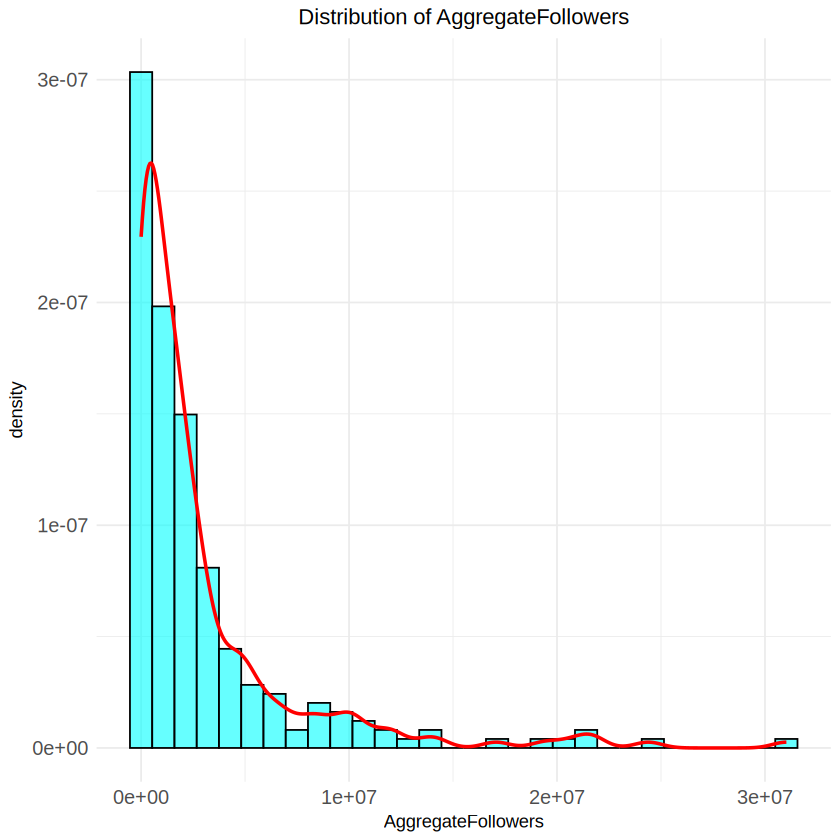
\includegraphics[width=0.75\columnwidth]{csm_figures/af_original_distribution.png}
    \caption{Phân phối ban đầu của Gross.}
    \label{fig:af_original_distribution}
\end{figure}
Nhận xét:
\begin{itemize}
    \item Nhìn vào biểu đồ, ta thấy phân phối của biến AggregateFollowers bị lệch phải.
\end{itemize}

\begin{figure}[H]
    \centering
    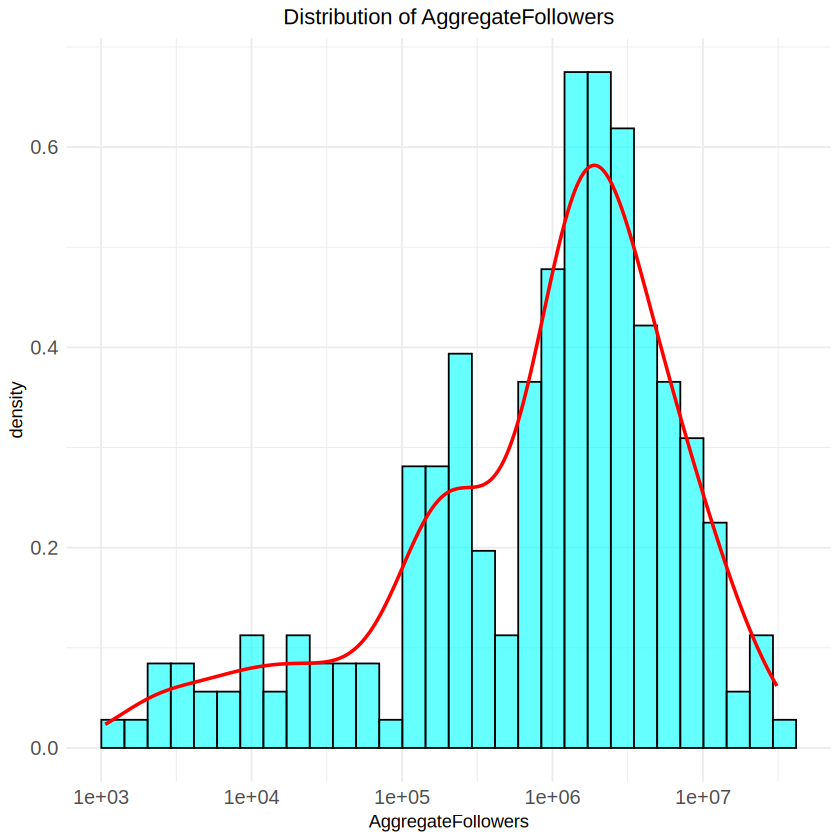
\includegraphics[width=0.75\columnwidth]{csm_figures/af_logscale_distribution.png}
    \caption{Phân phối sau khi logscale của AggregateFollowers.}
    \label{fig:af_logscale_distribution}
\end{figure}
Nhận xét:
\begin{itemize}
    \item Khi dùng log-scale, phân phối của biến Comments đã xấp xỉ chuẩn hơn.
    \item Ta có thể dùng box-cox để biến đổi dữ liệu nhờ vào việc tìm lambda tối ưu.
\end{itemize}

\begin{figure}[H]
    \centering
    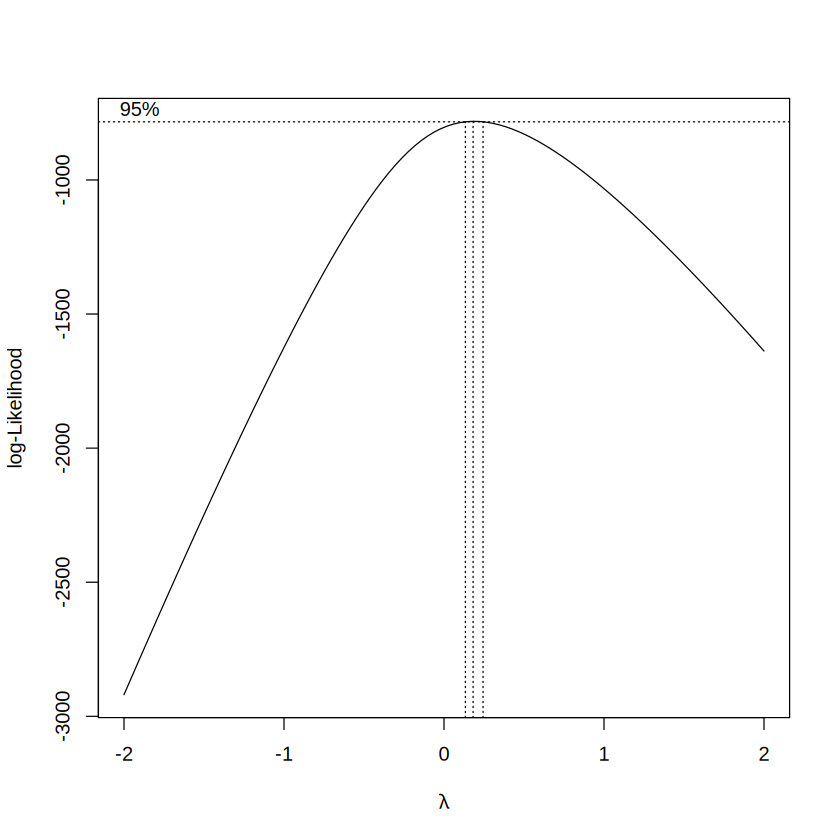
\includegraphics[width=0.75\columnwidth]{csm_figures/af_optimal_lambda.png}
    \caption{Log-likelihood với các giá trị $\lambda$ của AggregateFollowers.}
    \label{fig:af_optimal_lambda}
\end{figure}
Nhận xét:
\begin{itemize}
    \item Dựa trên biểu đồ, ta tìm được giá trị lambda tối ưu với mức ý nghĩa 5\% là 0.182
\end{itemize}

Và ta thực hiện biến đổi dữ liệu với giá trị lambda vừa tìm được.
\begin{figure}[H]
    \centering
    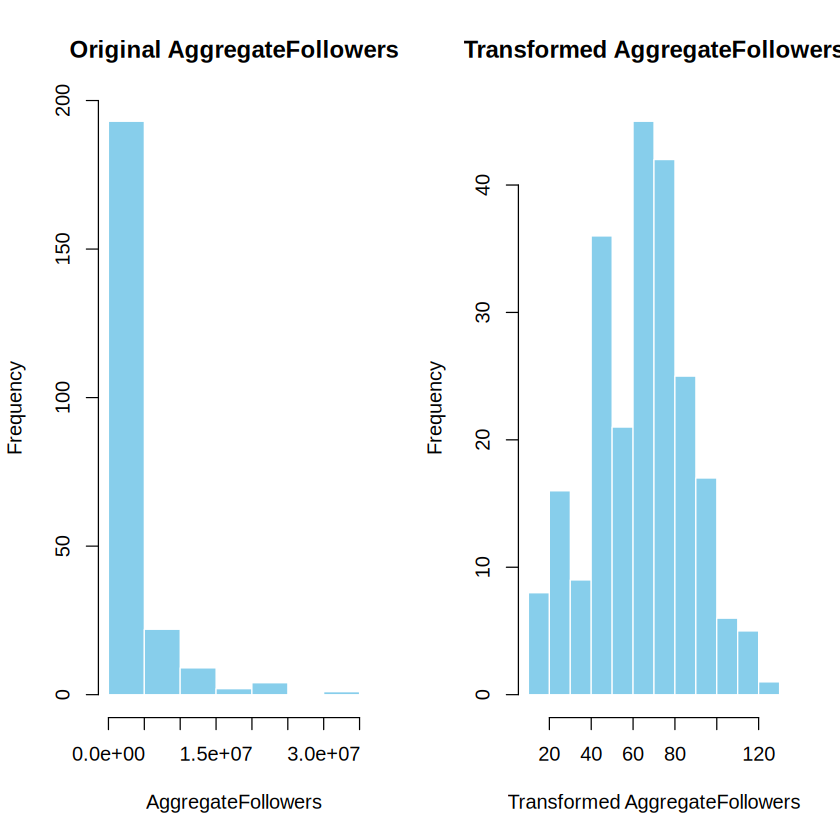
\includegraphics[width=0.75\columnwidth]{csm_figures/af_transformed_distribution.png}
    \caption{Phân phối trước và sau khi biến đổi của AggregateFollowers.}
    \label{fig:af_transformed_distribution}
\end{figure}
Nhận xét:
\begin{itemize}
    \item Ta có được giá trị lambda tối ưu là 0.33 và sử dụng giá trị này để biến đổi biến AggregateFollowers. Biểu đồ histogram phía bên dưới thể hiện phân phối của biến này trước và sau khi biến đổi. Dễ dàng thấy được, sau khi biến đổi, biến này đã tương đối chuẩn hơn.
\end{itemize}

\subsection{Mô hình hóa}

\subsubsection{Xử lý đa cộng tuyến}

Đầu tiên, ta trực quan hóa ma trận tương quan giữa các biến trong tập dữ liệu
\begin{figure}[H]
    \centering
    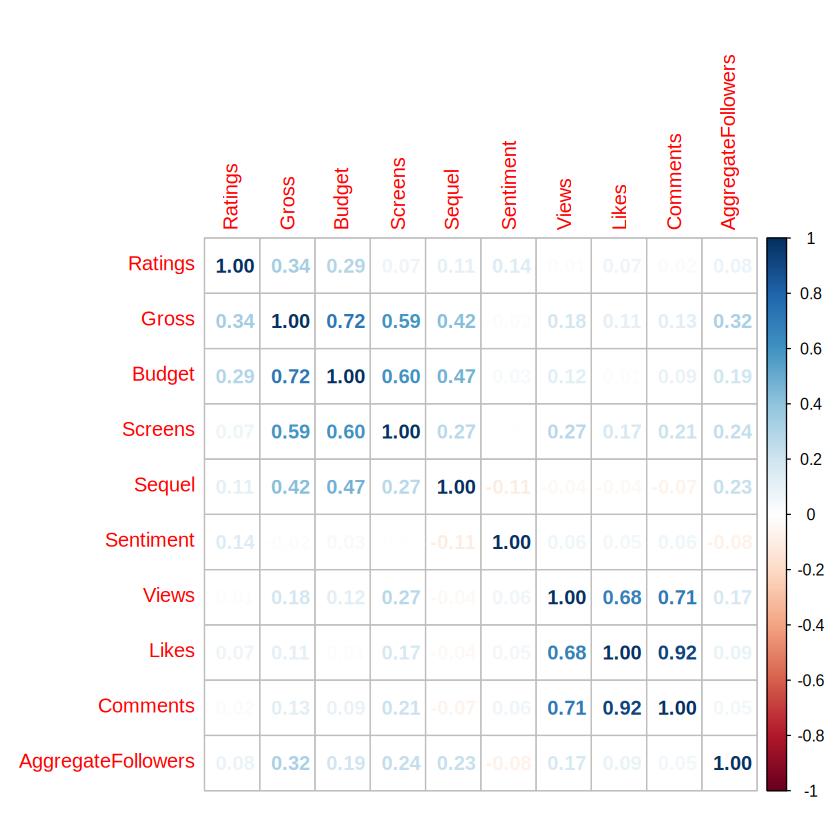
\includegraphics[width=0.75\columnwidth]{csm_figures/corr.png}
    \caption{Ma trận tương quan giữa các biến trong tập dữ liệu phim truyền thông.}
    \label{fig:csm_corr}
\end{figure}

Nhận xét:
\begin{itemize}
    \item Một số cặp có khả năng đa cộng tuyến cao: Views` và `Comments`, Likes` và `Comments`, `Gross` và `Budget`
    \item Một số cặp tương quan nghịch tương đối vừa: Sequel và Sentiment (-0.11)
\end{itemize}

Ta xử lý đa cộng tuyến thông qua các bước sau. Bước 1: Tính toán chỉ số VIF
\begin{lstlisting}
Ratings             Budget            Screens             Sequel 
          1.196619           2.239092           1.740774           1.406844 
         Sentiment              Views              Likes           Comments 
          1.050186           2.172907           7.324670           7.884851 
AggregateFollowers 
          1.147767 
\end{lstlisting}
Nhận xét:
\begin{itemize}
    \item Ta có chọn ngưỡng bằng 3
\end{itemize}
Bước 2: Loại bỏ các biến dựa trên VIF nếu vượt quá ngưỡng
\begin{lstlisting}
    Ratings             Budget            Screens             Sequel 
          1.152850           2.075596           1.736352           1.362376 
         Sentiment              Views              Likes AggregateFollowers 
          1.050070           2.007632           1.905291           1.129789 

Call:
lm(formula = Gross ~ Ratings + Budget + Screens + Sequel + Sentiment + 
    Views + Likes + AggregateFollowers, data = csm_df)

Residuals:
       Min         1Q     Median         3Q        Max 
-125889542  -27197502   -3079763   16371993  417347246 

Coefficients:
                     Estimate Std. Error t value Pr(>|t|)    
(Intercept)        -1.226e+08  2.671e+07  -4.588 7.50e-06 ***
Ratings             1.590e+07  4.005e+06   3.970 9.73e-05 ***
Budget              7.509e-01  9.803e-02   7.660 5.68e-13 ***
Screens             1.448e+04  3.372e+03   4.294 2.62e-05 ***
Sequel              8.854e+06  4.451e+06   1.989  0.04788 *  
Sentiment          -4.850e+05  5.402e+05  -0.898  0.37022    
Views               4.518e-01  1.158e+00   0.390  0.69692    
Likes               9.093e+01  1.766e+02   0.515  0.60717    
AggregateFollowers  2.494e+00  8.657e-01   2.880  0.00436 ** 
---
Signif. codes:  0 '***' 0.001 '**' 0.01 '*' 0.05 '.' 0.1 ' ' 1

Residual standard error: 55930000 on 222 degrees of freedom
Multiple R-squared:  0.6179,	Adjusted R-squared:  0.6042 
F-statistic: 44.88 on 8 and 222 DF,  p-value: < 2.2e-16
\end{lstlisting}
Như vậy, chúng ta đã thu được tập dữ liệu bao gồm các biến không có đa cộng tuyến với nhau. (Đã loại bỏ được biến comments)

\subsubsection{Khảo sát ngoại lai}

Để loại bỏ những ngoại lại, ta sử dụng IQR để tìm và loại bỏ các điểm cực ngoại lai.

\begin{lstlisting}
# Ở đây sử dụng IQR để loại bỏ ngoại lai
Q1 <- quantile(cleaned_df$'Gross', 0.25)
Q3 <- quantile(cleaned_df$'Gross', 0.75)
IQR <- Q3 - Q1
lower_bound <- Q1 - 1.5 * IQR
upper_bound <- Q3 + 1.5 * IQR
outliers <- which(cleaned_df$'Gross' < lower_bound | cleaned_df$'Gross' > upper_bound)
print(outliers)

lower_bound <- Q1 - 3 * IQR
upper_bound <- Q3 + 3 * IQR
extreme_outliers <- which(cleaned_df$'Gross' < lower_bound | cleaned_df$'Gross' > upper_bound)
print(extreme_outliers)
\end{lstlisting}

Ta thu được các điểm dữ liệu ngoại lai: 11  19  27  28  47  71 125 128 134 151 162 164 165 166 167 168

Các điểm dữ liệu cực ngoại lai: 11  47 128 164 165 166 167

Bằng cách loại bỏ các điểm dữ liệu cực ngoại lai, ta thu được tập dữ liệu để có thể khảo sát tiếp.


\subsubsection{Xây dựng mô hình đầy đủ}

Đầu tiên, ta phân chia tập dữ liệu thành 2 phần: train (80\%) và test (20\%).
\begin{lstlisting}
split_ratio <- 0.8
split_index <- floor(nrow(csm_df) * split_ratio)

train = csm_df[1:split_index,]
test = csm_df[(split_index + 1):nrow(csm_df),]
\end{lstlisting}

Sau đó, ta xây dựng mô hình đầy đủ các biến như sau:

\begin{lstlisting}
full.lm <- lm(Gross ~ ., data = train)
print(summary(full.lm))
\end{lstlisting}

Kết quả

\begin{lstlisting}
lm(formula = Gross ~ ., data = train)

Residuals:
    Min      1Q  Median      3Q     Max 
-136.99  -18.79    3.70   22.97   84.15 

Coefficients:
                    Estimate Std. Error t value Pr(>|t|)    
(Intercept)        -60.21332   62.87576  -0.958   0.3396    
Ratings             21.80737   12.55030   1.738   0.0841 .  
Budget               0.65118    0.08619   7.555 2.46e-12 ***
Screens              2.89668    0.49989   5.795 3.25e-08 ***
Sequel              11.31840    6.07145   1.864   0.0640 .  
Sentiment           -0.21697   10.96256  -0.020   0.9842    
Views               -0.29107    0.25634  -1.136   0.2578    
Likes                1.79341    0.75762   2.367   0.0190 *  
AggregateFollowers   0.03477    0.09788   0.355   0.7228    
---
Signif. codes:  0 '***' 0.001 '**' 0.01 '*' 0.05 '.' 0.1 ' ' 1

Residual standard error: 34.9 on 170 degrees of freedom
Multiple R-squared:  0.6614,	Adjusted R-squared:  0.6455 
F-statistic: 41.51 on 8 and 170 DF,  p-value: < 2.2e-16
\end{lstlisting}
Nhận xét:
\begin{itemize}
    \item Mô hình này có R-squared hiệu chỉnh 0.6455, tức là phương sai biến Gross có thể được giải thích được 64.55\% dựa trên các biến độc lập của mô hình.
    \item Với mức ý nghĩa 5\%, ta thấy các biến Budget, Screen, Ratings, Sequel và Likes có ý nghĩa đối với mô hình
\end{itemize}

\subsubsection{Lựa chọn model tốt nhất}

Với số lượng lớn các yếu tố dự đoán, điều quan trọng là phải giảm thiểu mô hình bằng cách chỉ bao gồm các yếu tố dự đoán hữu ích. Có tất cả 8 yếu tố dự đoán trong tập dữ liệu, nghĩ là có thể có $2^{8}$ mô hình hồi quy. Để chọn mô hình một cách hiệu quả, việc lựa chọn lùi được thực hiện bằng sử dụng step function. Phương pháp này lặp lại các quy trình để giảm thiểu Akaike’s Information Criteria (AIC) và Bayesian Information Criteria (BIC). Lựa chọn mô hình ngược so với lựa chọn tiến vì nó loại bỏ khả năng một yếu tố dự đoán mới được chọn có khả năng tương tự hoặc nhiều hơn để giải thích các phần của phản hồi đã được giải thích bởi một yếu tố dự đoán khác có trong mô hình.

\begin{lstlisting}
# Mô hình chặn dưới
model.lb <- lm(Gross ~ 1, data = train) 

# Mô hình chặn trên
model.up <- full.lm

step(full.lm, scope = list(lower = model.lb, upper = model.up), direction = "both", trace = FALSE)
\end{lstlisting}

Kết quả
\begin{lstlisting}
Call:
lm(formula = Gross ~ Ratings + Budget + Screens + Sequel + Likes, 
    data = train)

Coefficients:
(Intercept)      Ratings       Budget      Screens       Sequel        Likes  
   -72.5562      24.4101       0.6444       2.9817      11.9940       1.0309  
\end{lstlisting}

\begin{lstlisting}
csm_models<- regsubsets(Gross ~  Ratings + Dislikes + AggregateFollowers, data = train)
summary.csm<-summary(csm_models)

# Lựa chọn mô hình tốt nhất từ reg subsets 
summary.csm$which
\end{lstlisting}


Xây dựng mô hình tốt nhất dựa trên BIC

\begin{lstlisting}
# Tiêu chí chọn mô hình tốt nhất 4: mô hình với BIC nhỏ
summary.csm$bic

best_model_index <- which.min(summary.csm$bic)
best_model <- summary.csm$which[best_model_index, ]
print(best_model)
best_vars <- names(best_model[best_model])
best_vars <- best_vars[best_vars != "(Intercept)"]
print(best_vars)

# Xây dựng mô hình tốt nhất
formula_str <- paste("Gross ~", paste(best_vars, collapse = " + "))
best_model_csm <- lm(as.formula(formula_str), data=train)

# Tóm tắt mô hình
summary(best_model_csm)
\end{lstlisting}

Kết quả:
\begin{lstlisting}
lm(formula = as.formula(formula_str), data = train)

Residuals:
     Min       1Q   Median       3Q      Max 
-142.604  -17.715    1.929   22.419   87.326 

Coefficients:
             Estimate Std. Error t value Pr(>|t|)    
(Intercept) -27.97801   10.72422  -2.609 0.009870 ** 
Budget        0.75150    0.07662   9.808  < 2e-16 ***
Screens       2.78579    0.48627   5.729 4.33e-08 ***
Likes         1.02351    0.29564   3.462 0.000674 ***
---
Signif. codes:  0 '***' 0.001 '**' 0.01 '*' 0.05 '.' 0.1 ' ' 1

Residual standard error: 35.3 on 175 degrees of freedom
Multiple R-squared:  0.6434,	Adjusted R-squared:  0.6373 
F-statistic: 105.3 on 3 and 175 DF,  p-value: < 2.2e-16
\end{lstlisting}
Như vậy, ta thu được mô hình
\begin{equation}
    \text{Gross ~ -27.97801 * (Intercept) + 0.75150 * Budget + 2.78579 * Screens * 1.02351 * Likes}
\end{equation}
Nhận xét:
\begin{itemize}
    \item R-squared hiệu chỉnh của mô hình là 0.6373, tức là 63.73\% phương sai của biến  Gross được giải thích bởi các biến độc lập của mô hình được chọn.
    \item Điều này có ý nghĩa là, biến Gross sẽ được giải thích thông qua hai biến Budget, Screens và Likes 
    \item Số lượng rạp chiếu có ảnh hưởng nhiều đến với tổng doanh thu của một bộ phim. Số lượng rạp chiếu càng nhiều thì doanh thu của một bộ phim càng cao.
    \item Số lượt thích của một bộ phim cũng ảnh hưởng đến tổng doanh thu của một bộ phim. Một bộ phim được nhiều người yêu thích thì doanh thu càng cao.
\end{itemize}

Bây giờ, ta sẽ đi phân tích mô hình này. 
\begin{figure}[H]
    \centering
    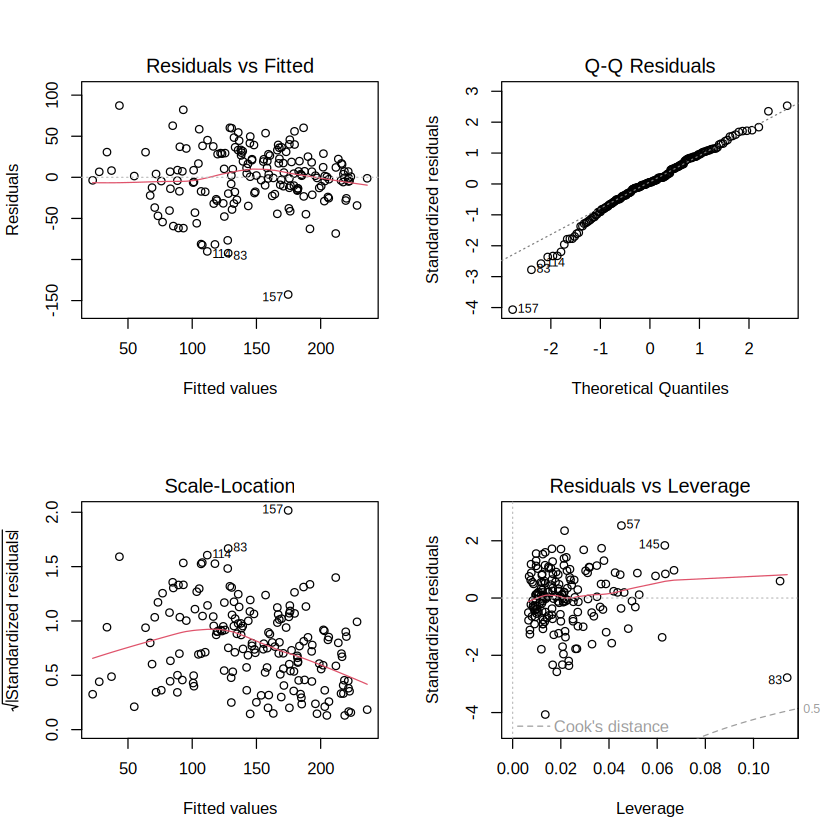
\includegraphics[width=0.75\columnwidth]{csm_figures/best_csm_model.png}
    \caption{.}
    \label{fig:best_csm_model}
\end{figure}

\textbf{Phân tích Residuals vs Fitted Plot}: Biểu đồ Residuals vs Fitted Plot đưa ra dấu hiệu nếu có các mẫu phi tuyến tính. Để hồi quy tuyến tính chính xác, dữ liệu cần phải tuyến tính nên điều này sẽ kiểm tra xem điều kiện đó có được đáp ứng hay không.

\begin{figure}[H]
    \centering
    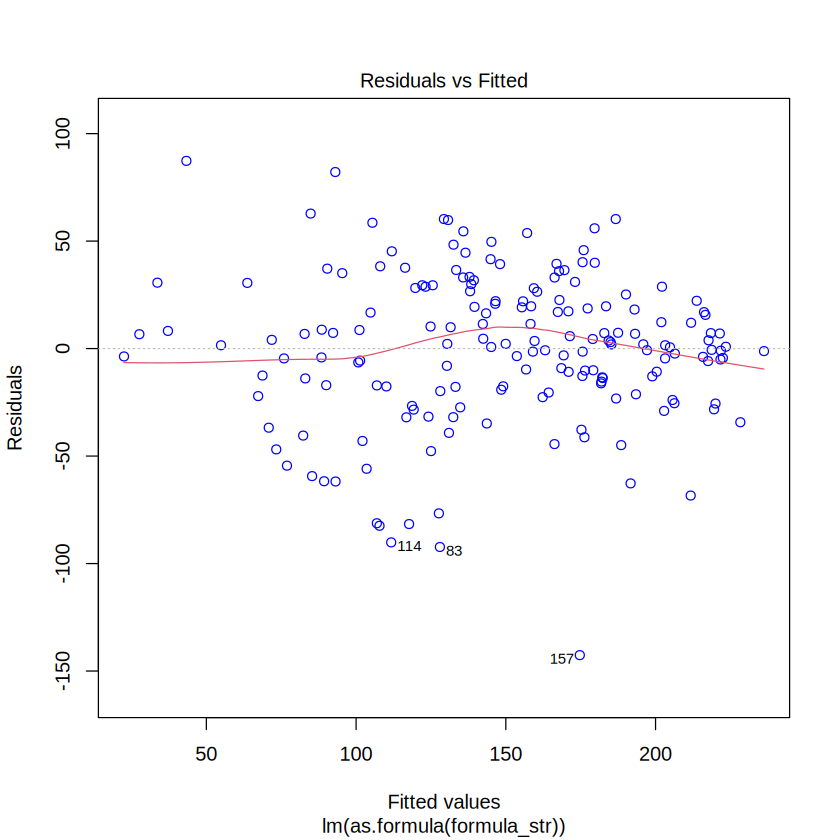
\includegraphics[width=0.75\columnwidth]{csm_figures/best_csm_model_residual_fitted.png}
    \caption{Biểu đồ Residuals vs Fitted Plot.}
    \label{fig:best_model_fig2}
\end{figure}

Dựa trên biểu đồ này, ta thấy đường cong màu đỏ có dáng gần như một đường thẳng, và các phần tử trải dọc theo đường cong này một cách tương đồng đều. Điều này chứng tỏ không có quan hệ phi tuyến xuất hiện trong dữ liệu.

\textbf{Phân tích Normal Q–Q (quantile-quantile) Plot}: Các giá trị thặng dư (residual) nên có phân phối chuẩn. Để kiểm tra điều này, chúng ta cần quan sát biểu đồ QQ Residuals plot, nếu các điểm được xếp thành một đường thẳng (hoặc gần như thẳng) thì chứng tỏ các giá trị thặng dư (residual) có phân phối chuẩn.

\begin{figure}[H]
    \centering
    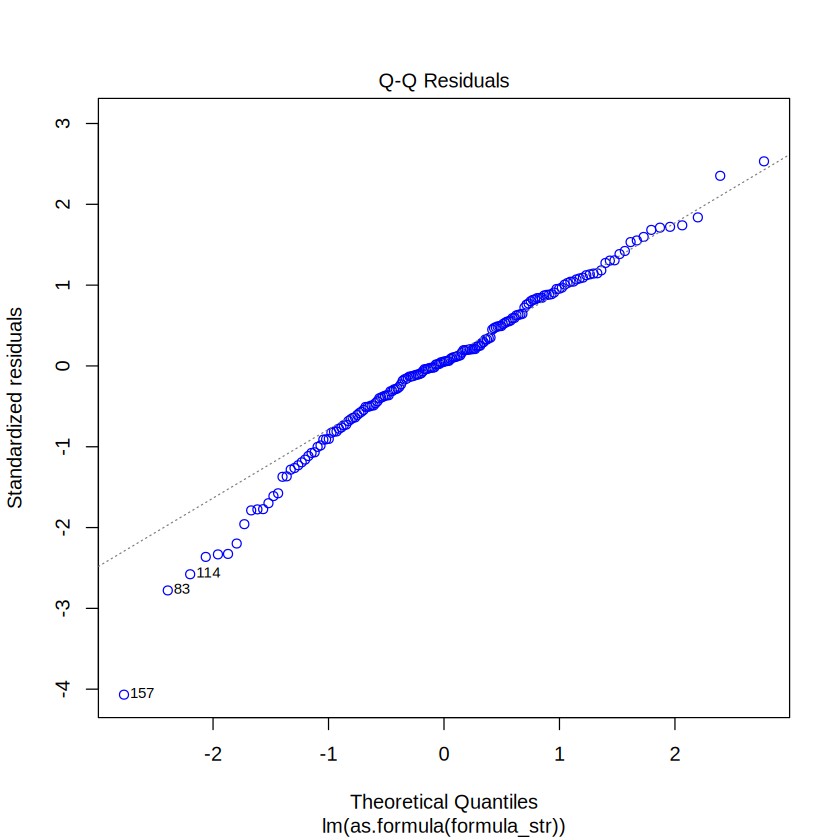
\includegraphics[width=0.75\columnwidth]{csm_figures/best_csm_model_qq.png}
    \caption{Normal Q–Q (quantile-quantile) Plot.}
    \label{fig:best_csm_model_qq}
\end{figure}

Như hình vẽ kết quả ở trên, ta thấy rõ điều đó, residual có phân phối chuẩn.

Cẩn thận hơn, chúng ta thử dùng Shapiro–Wilk test để kiểm tra có đúng thật là các giá trị thặng dư có phân phối chuẩn hay không?
\begin{itemize}
    \item H0: Biến thặng dư của mô hình phân phối chuẩn trong một số quần thể.
    \item H1: Biến thặng dư của mô hình không phân phối chuẩn trong một số quần thể.
\end{itemize}

Kết quả:
\begin{lstlisting}
Shapiro-Wilk normality test

data:  model$residuals
W = 0.97565, p-value = 0.003158

[1] "H0 rejected: the residuals are NOT distributed normally"
\end{lstlisting}

Kết quả cho thấy p-value bé hơn mức ý nghĩa alpha 0.05 nên ta có thể bác bỏ giả thhuyết H0, biến thặng dư của chúng ta không chuẩn trong một số quần thể.  

\begin{figure}[H]
    \centering
    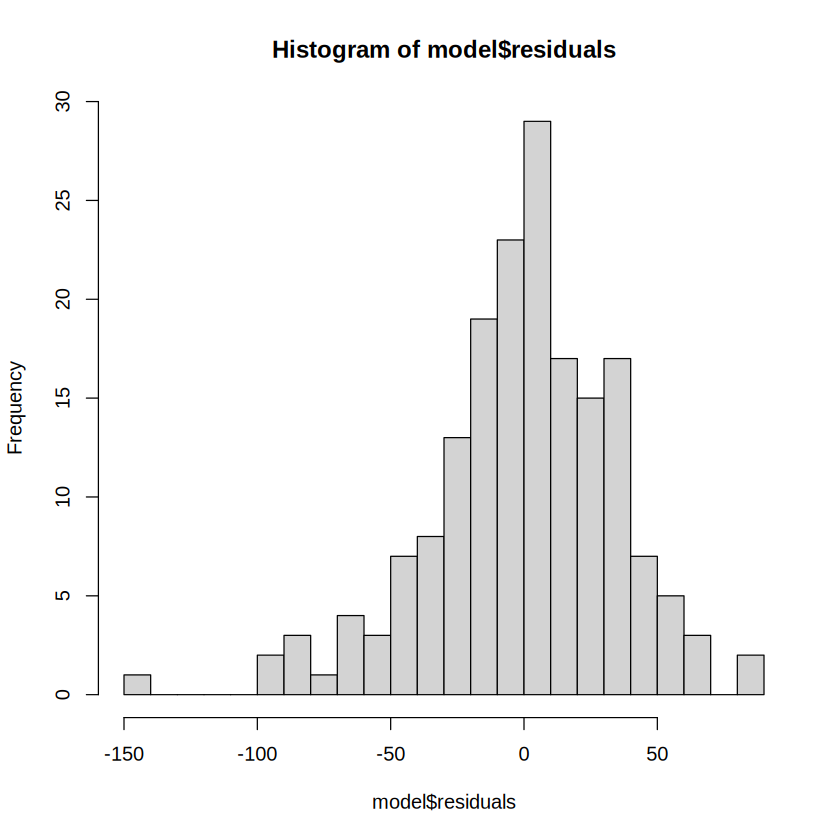
\includegraphics[width=0.75\columnwidth]{csm_figures/best_csm_model_qq2.png}
    \caption{Histogram biến thặng dư của mô hình hồi quy CSM.}
    \label{fig:best_csm_model_qq2}
\end{figure}

\textbf{Phân tích Scale-Location}: Biểu đồ scale-location kiểm định giả định hồi quy về phương sai bằng nhau (homoscedasticity), tức là giá trị thặng dư có phương sai bằng với đường hồi quy.

\begin{figure}[H]
    \centering
    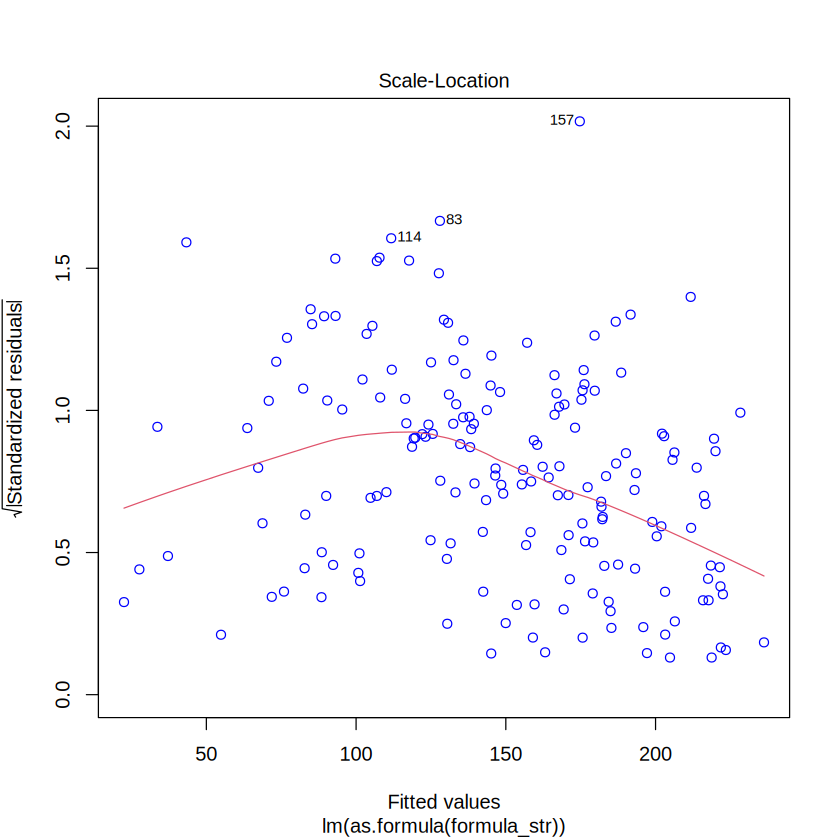
\includegraphics[width=0.75\columnwidth]{csm_figures/best_csm_model_scale.png}
    \caption{Scale-Location Plot.}
    \label{fig:best_csm_model_scale}
\end{figure}
Nhận xét:
\begin{itemize}
    \item Đường màu đỏ gần bị lệch về phía dưới của biểu đồ. Nghĩa là, độ phân tán của giá trị thặng dư gần không bằng nhau ở tất cả các giá trị phù hợp. 
    \item  Các giá trị thặng dư được phân tán ngẫu nhiên xung quanh đường màu đỏ với độ biến thiên tương đối bằng nhau ở tất cả các giá trị phù hợp.
\end{itemize}

Cẩn thận hơn, chúng ta sử dụng Breusch-Pagan test để kiểm tra có thật là như vậy không?
\begin{itemize}
    \item H0: Các giá trị thặng dư là homoscedastic
    \item H1: Các giá trị thặng dư là heteroscedastic
\end{itemize}
Kết quả:
\begin{lstlisting}
studentized Breusch-Pagan test

data:  model
BP = 6.8056, df = 3, p-value = 0.07836

[1] "H0 failed to reject: Error variance spreads CONSTANTLY (Homoscedasticity)"
\end{lstlisting}

Như vậy, ta thấy p-value lớn hơn múc ý nghĩa 0.05, ta chưa đủ điều kiện bác bỏ H0. Vậy các giá trị thặng dư là homoscedastic

\textbf{Phân tích Residuals vs Leverage} Biểu đồ này có thể được sử dụng để tìm các trường hợp có ảnh hưởng trong tập dữ liệu. Một trường hợp có ảnh hưởng là một trường hợp mà nếu bị loại bỏ sẽ ảnh hưởng đến mô hình nên việc đưa vào hoặc loại trừ nó cần được xem xét.

Một trường hợp có ảnh hưởng có thể là một trường hợp ngoại lệ hoặc không và mục đích của biểu đồ này là xác định các trường hợp có ảnh hưởng lớn đến mô hình. Các ngoại lệ sẽ có xu hướng có giá trị cực cao hoặc cực thấp và do đó ảnh hưởng đến mô hình.

\begin{figure}[H]
    \centering
    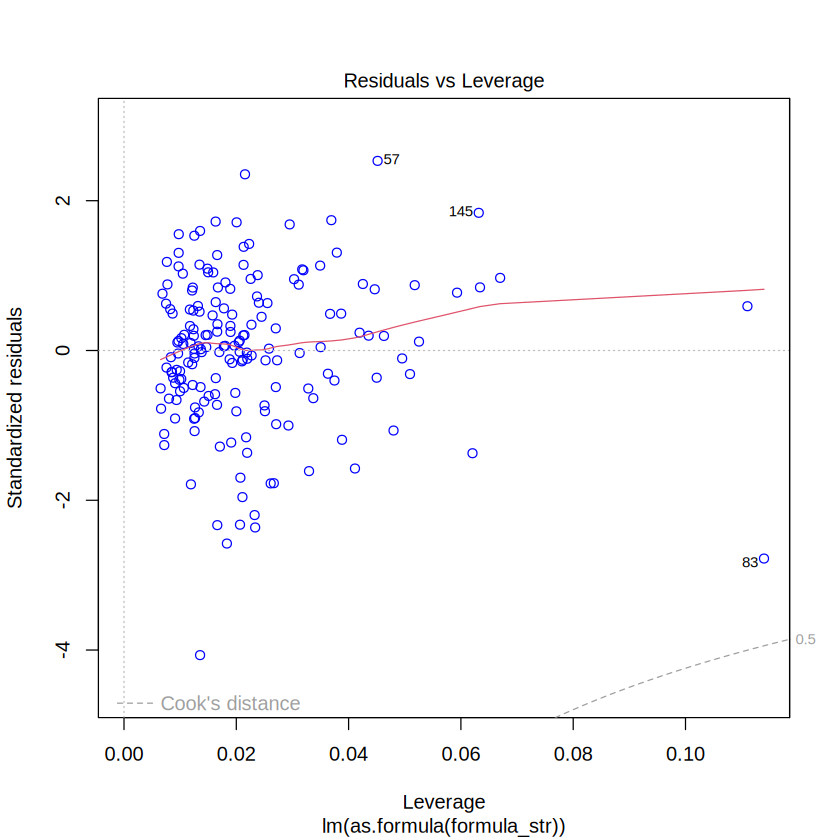
\includegraphics[width=0.75\columnwidth]{csm_figures/best_csm_model_residual_leverage.png}
    \caption{Residuals vs Leverage Plot.}
    \label{fig:best_csm_model_residual_leverage}
\end{figure}
Nhận xét:
\begin{itemize}
    \item Một số điểm như 57, 83, 145 có thể là các điểm ngoại lai. Ta có thể thử loại bỏ để nâng cao chất lượng mô hình.
\end{itemize}

Ta cũng có thể nhận thấy có một số giá trị ngoại lai ở cách xa đường thằng giữa. Ta có thể xem rõ hơn thông qua histogram của Cook's Distance
\begin{figure}[H]
    \centering
    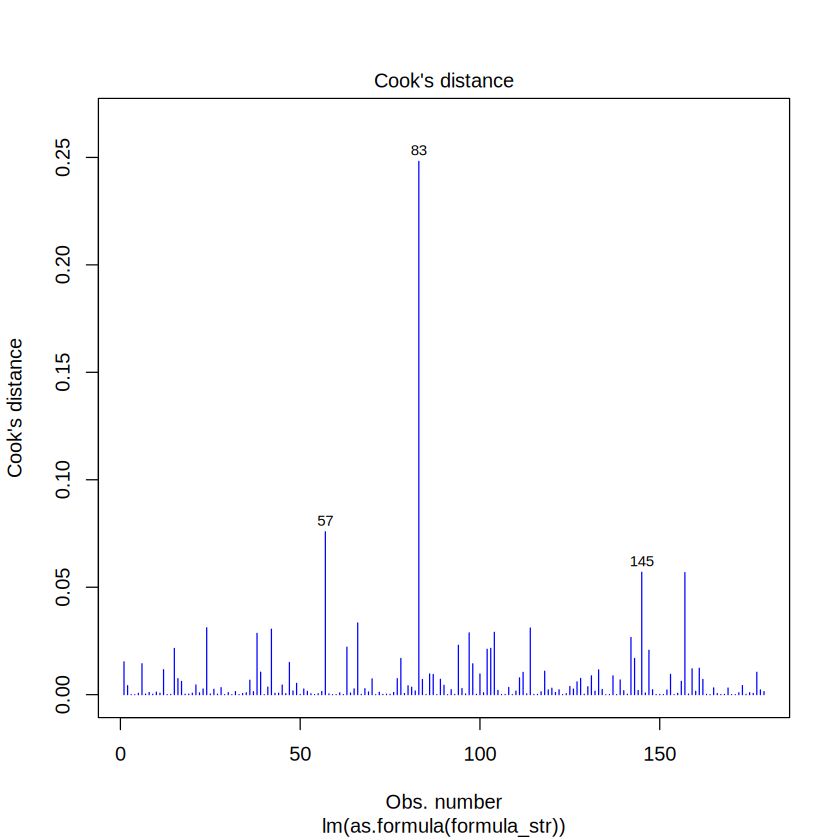
\includegraphics[width=0.75\columnwidth]{csm_figures/best_csm_model_cook.png}
    \caption{Cook Distance Plot của mô hình hồi quy CSM.}
    \label{fig:best_csm_model_cook}
\end{figure}

\subsubsection{Loại bỏ ngoại lai dựa trên Cook'Distance}

Sau khi loại bỏ những điểm có tiềm năng là ngoại lai, ta thu được các mô hình. Dựa trên các tiêu chí và R-squared hiệu chỉnh, đánh giá kiểm định phần thặng dư và đồng nhất phương sai. Ta vẫn lựa chọn được mô hình khi loại bỏ vừa đủ các điểm tiềm năng (Xem file code).

\begin{lstlisting}
lm(formula = as.formula(formula_str), data = train[-c(influential_points), 
    ])

Residuals:
   Min     1Q Median     3Q    Max 
-71.07 -17.18   0.42  19.32  58.85 

Coefficients:
             Estimate Std. Error t value Pr(>|t|)    
(Intercept) -21.37468    9.25407  -2.310   0.0222 *  
Budget        0.65659    0.06692   9.811  < 2e-16 ***
Screens       3.27610    0.41667   7.863 4.99e-13 ***
Likes         1.14767    0.25277   4.540 1.09e-05 ***
---
Signif. codes:  0 '***' 0.001 '**' 0.01 '*' 0.05 '.' 0.1 ' ' 1

Residual standard error: 27.76 on 162 degrees of freedom
Multiple R-squared:  0.7377,	Adjusted R-squared:  0.7329 
F-statistic: 151.9 on 3 and 162 DF,  p-value: < 2.2e-16
\end{lstlisting}
Nhận xét:
\begin{itemize}
    \item R-squared hiệu chỉnh của mô hình là 0.7329, có nghĩa là 73.29\% phương sai của Gross có thể được giải thích bởi các biến độc lập của mô hình.
\end{itemize}

Kiểm định phân phối chuẩn cho biến thặng dư. Ta có kết quả như sau:
\begin{lstlisting}
Shapiro-Wilk normality test

data:  model$residuals
W = 0.98973, p-value = 0.2725

[1] "H0 failed to reject: the residuals ARE distributed normally"
\end{lstlisting}
Kết quả cho thấy p-value lớn hơn mức ý nghĩa alpha 0.05 nên ta có thể bác bỏ giả thhuyết H0, biến thặng dư của chúng ta chuẩn trong một số quần thể.  

Và kiểm định đồng nhất phương sai. Ta có kết quả:
\begin{lstlisting}
studentized Breusch-Pagan test

data:  model
BP = 11.356, df = 3, p-value = 0.009948

[1] "H0 rejected: Error variance spreads INCONSTANTLY/generating patterns (Heteroscedasticity)"
\end{lstlisting}
Như vậy, ta thấy p-value nhỏ hơn múc ý nghĩa 0.05, ta chưa đủ điều kiện bác bỏ H0. Vậy các giá trị thặng dư là heteroscedasticity

\subsubsection{Dự đoán và đánh giá kết quả}

Ta trực quan kết quả dự đoán và đánh giá RMSE của mô hình đã chọn.

\begin{figure}[H]
    \centering
    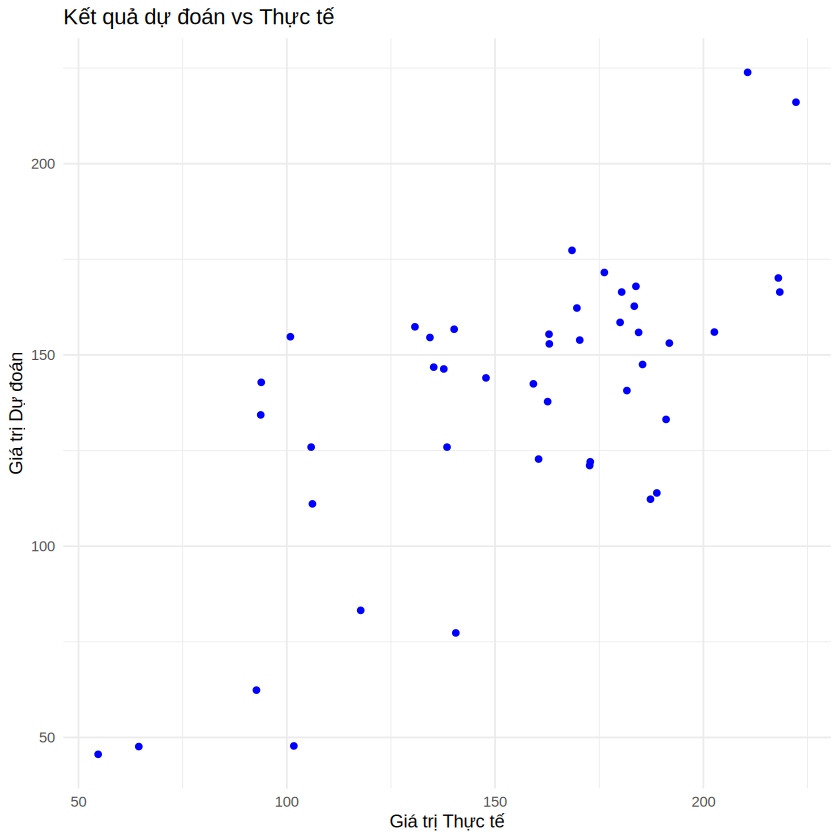
\includegraphics[width=0.75\columnwidth]{csm_figures/prediction_model_best.png}
    \caption{Trực quan kết quả dự đoán của mô hình tốt nhất. RMSE = 196.83.}
    \label{fig:prediction_model_best}
\end{figure}

Hiệu suất trên các độ đo:
\begin{itemize}
    \item "MSE: 1231.319394"
    \item "RMSE: 35.090161"
    \item "MAE: 28.99513"
    \item "Correlation: 0.694378"
    \item "R\^2 between y\_pred \& y\_true: 0.482161"
\end{itemize}

\subsection{Mô hình hóa bằng PCR}

Principal Component Regression (PCR) là một kỹ thuật kết hợp Phân tích thành phần chính (PCA) và hồi quy tuyến tính để giải quyết đa cộng tuyến và giảm chiều trong các tập dữ liệu cao chiều. Các bước chính trong PCR là:
\begin{itemize}
    \item PCA biến đổi các biến dự báo ban đầu thành một tập hợp các biến mới, không tương quan được gọi là các thành phần chính. Các thành phần này là các tổ hợp tuyến tính của các biến ban đầu và được sắp xếp theo lượng phương sai mà chúng giải thích trong dữ liệu. Mỗi thành phần chính nắm bắt được phương sai tối đa có thể trong khi vẫn trực giao với các thành phần trước đó.
    \item Một tập hợp con các thành phần chính (giải thích phương sai lớn nhất) được chọn và sử dụng làm các yếu tố dự báo trong mô hình hồi quy tuyến tính để dự báo biến phản hồi. Bằng cách tập trung vào các thành phần chính nắm bắt được phương sai lớn nhất, PCR hướng đến mục tiêu xây dựng một mô hình hồi quy ổn định và dễ diễn giải hơn.
\end{itemize}

\begin{lstlisting}
pcr_model <- pcr(`Gross` ~ ., data = train, scale = TRUE, validation = "CV") # Fit PCR model with cross-validation
\end{lstlisting}

Đối số xác thực = “CV” chỉ định rằng xác thực chéo (cross-validation - CV) nên được sử dụng để xác thực mô hình. Xác thực chéo là một phương pháp mạnh mẽ để đánh giá hiệu suất dự đoán của một mô hình. Nó bao gồm việc phân vùng dữ liệu thành các tập hợp con, huấn luyện mô hình trên một số tập hợp con (bộ huấn luyện - training set) và xác thực nó trên các tập hợp con còn lại (bộ xác thực - validation set). Quá trình này được lặp lại nhiều lần để đảm bảo hiệu suất của mô hình là nhất quán và không phụ thuộc vào phân vùng dữ liệu cụ thể.

Bằng cách sử dụng xác thực chéo, mô hình ít có khả năng quá khớp với dữ liệu huấn luyện. Quá khớp xảy ra khi mô hình nắm bắt được nhiễu và các mẫu cụ thể trong dữ liệu huấn luyện không tổng quát hóa thành dữ liệu mới, chưa từng thấy. Xác thực chéo giúp phát hiện và giảm thiểu tình trạng quá khớp bằng cách kiểm tra mô hình trên các tập hợp con khác nhau của dữ liệu.

\begin{lstlisting}
Data: 	X dimension: 184 9 
	Y dimension: 184 1
Fit method: svdpc
Number of components considered: 9

VALIDATION: RMSEP
Cross-validated using 10 random segments.
       (Intercept)  1 comps  2 comps  3 comps  4 comps  5 comps  6 comps
CV           61.54    50.28    39.01    38.64    36.10    35.65    36.19
adjCV        61.54    50.21    39.01    38.64    36.03    35.53    36.10
       7 comps  8 comps  9 comps
CV       36.42    36.61    36.68
adjCV    36.32    36.49    36.54

TRAINING: % variance explained
       1 comps  2 comps  3 comps  4 comps  5 comps  6 comps  7 comps  8 comps
X        36.99    56.35    69.36    79.30    87.38    94.55    98.22    99.47
Gross    34.19    61.29    62.20    67.11    68.00    68.02    68.39    68.44
       9 comps
X       100.00
Gross    69.01
\end{lstlisting}

\textbf{Lựa chọn số lượng thành phần chính}: Để quyết định được số thành phần chính tối ưu, chúng ta cần phải trung hòa giữa độ phức tạp của mô hình (tức là số lượng components) và RMSEP (Root Mean Squared Error of Prediction).

\begin{figure}[H]
    \centering
    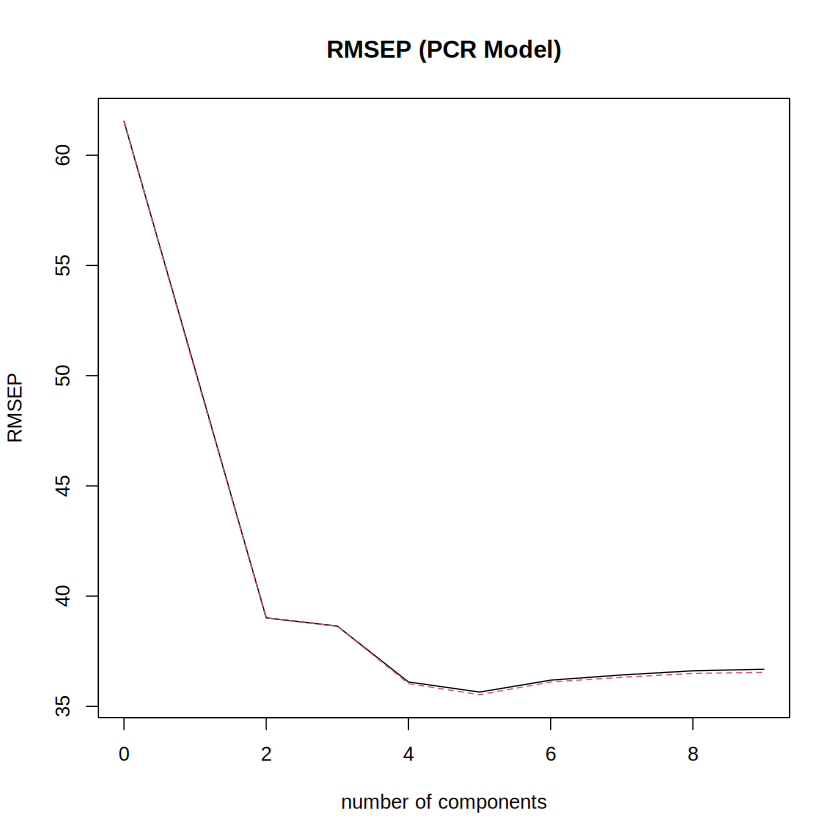
\includegraphics[width=0.75\columnwidth]{csm_figures/pcr_part01.png}
    \caption{Giá trị RMSEP với số lượng thành phần chính khác nhau.}
    \label{fig:pcr_part01}
\end{figure}

\begin{itemize}
    \item RMSEP Values: 5 components - 35.53 (nhỏ nhất)
    \item Variance Explained: 5 components - 68.00\%
\end{itemize}
Do đó ta chọn 5 components.

\textbf{Đánh giá kết quả dự đoán}

\begin{figure}[H]
    \centering
    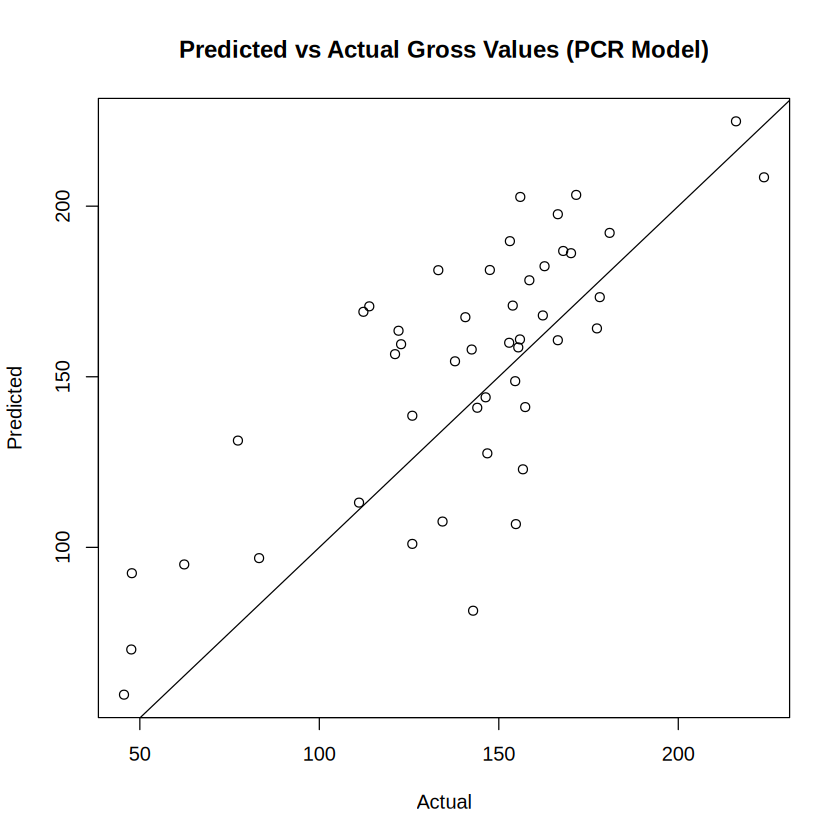
\includegraphics[width=0.75\columnwidth]{csm_figures/pcr_predict_part01.png}
    \caption{Kết quả dự đoán của mô hình PCR.}
    \label{fig:pcr_predict_part01}
\end{figure}

\begin{lstlisting}
# Calculate and print the Root Mean Squared Error (RMSE)
rmse <- sqrt(mean((test$`Gross` - predictions)^2))  # Calculate RMSE between actual and predicted values
print(paste("RMSE: ", rmse)) 
\end{lstlisting}

Kết quả: RMSE:  29.0363826627182

\begin{lstlisting}
# Calculate the sum of squares of residuals
ss_res <- sum((test$`Gross` - predictions)^2)

# Calculate the total sum of squares
ss_tot <- sum((test$`Gross` - mean(test$`Gross`))^2)

# Calculate R-squared
r_squared <- 1 - (ss_res / ss_tot)

# Print R-squared
print(paste("R-squared: ", r_squared))
\end{lstlisting}

Kết quả: 0.418260507745999

Giá trị R-squared 0.4182 có nghĩa là 41.82\% phương sai của biến phụ thuộc Gross được giải thích bởi các biến độc lập của mô hình.

Kiểm định thặng dư và đồng nhất phương sai cho kết quả:
\begin{lstlisting}
Shapiro-Wilk normality test

data:  model$residuals
W = 0.98315, p-value = 4.99e-13

[1] "H0 rejected: the residuals are NOT distributed normally"
\end{lstlisting}
Nhận xét:
\begin{itemize}
    \item Mô hình thỏa mãn giả định phân phối thặng dư không xấp xỉ chuẩn
\end{itemize}
\begin{figure}[H]
    \centering
    \includegraphics[width=0.75\columnwidth]{csm_figures/pcr_normality_test.png}
    \caption{Kiểm định tính chuẩn thặng dư của mô hình PCR.}
    \label{fig:pcr_normality_test}
\end{figure}

\begin{lstlisting}
studentized Breusch-Pagan test

data:  model
BP = 16.065, df = 9, p-value = 0.06554

[1] "H0 failed to reject: Error variance spreads CONSTANTLY (Homoscedasticity)"
\end{lstlisting}
\begin{itemize}
    \item Mô hình không đồng nhất phương sai
\end{itemize}
\begin{figure}[H]
    \centering
    \includegraphics[width=0.75\columnwidth]{csm_figures/pcr_homo_test.png}
    \caption{Kiểm định đồng nhất phương sai của mô hình PCR.}
    \label{fig:pcr_homo_test}
\end{figure}

\subsection{Mô hình hóa bằng PLS}

Partial Least Squares Regression là một kỹ thuật, không giống như PCR, xem xét cả các biến dự báo và biến phản hồi trong quá trình giảm chiều. Các bước chính trong PLS là:
\begin{itemize}
    \item Latent Variable Extraction: PLS trích xuất một tập hợp các biến tiềm ẩn (thành phần) tối đa hóa hiệp phương sai giữa các biến dự báo và biến phản hồi. Các thành phần này là các tổ hợp tuyến tính của các biến ban đầu, được chọn theo cách mà chúng nắm bắt được càng nhiều thông tin có liên quan càng tốt để dự đoán biến phản hồi. Điều này đảm bảo rằng các thành phần được trích xuất có liên quan trực tiếp đến kết quả quan tâm.
    \item Regression: Các biến tiềm ẩn sau đó được sử dụng làm biến dự báo trong mô hình hồi quy tuyến tính để dự báo biến phản hồi. Bằng cách kết hợp biến phản hồi vào quy trình trích xuất thành phần, PLS hướng đến mục tiêu cải thiện độ chính xác dự báo của mô hình hồi quy.
\end{itemize}

\begin{lstlisting}
Data: 	X dimension: 184 9 
	Y dimension: 184 1
Fit method: kernelpls
Number of components considered: 9

VALIDATION: RMSEP
Cross-validated using 10 random segments.
       (Intercept)  1 comps  2 comps  3 comps  4 comps  5 comps  6 comps
CV           61.54    39.76    36.29    36.20    36.70    36.84    37.03
adjCV        61.54    39.71    36.22    36.12    36.58    36.71    36.88
       7 comps  8 comps  9 comps
CV       37.20    37.15    37.11
adjCV    37.03    36.98    36.95

TRAINING: % variance explained
       1 comps  2 comps  3 comps  4 comps  5 comps  6 comps  7 comps  8 comps
X        33.56    55.01    66.00    73.38    81.48    86.81    91.62    94.29
Gross    59.95    67.52    68.43    68.62    68.75    68.91    69.00    69.01
       9 comps
X       100.00
Gross    69.01
\end{lstlisting}

\textbf{Lựa chọn số lượng thành phần chính}: Để quyết định được số thành phần chính tối ưu, chúng ta cần phải trung hòa giữa độ phức tạp của mô hình (tức là số lượng components) và RMSEP (Root Mean Squared Error of Prediction).

\begin{figure}[H]
    \centering
    \includegraphics[width=0.75\columnwidth]{csm_figures/pls_part01.png}
    \caption{Giá trị RMSEP với số lượng thành phần chính khác nhau.}
    \label{fig:pls_part01}
\end{figure}

\begin{itemize}
    \item RMSEP Values: 2 components - 36.22
    \item Variance Explained: 3 components - 67.52\% 
\end{itemize}
Do đó ta chọn 2 components.

\textbf{Đánh giá kết quả dự đoán}

\begin{figure}[H]
    \centering
    \includegraphics[width=0.75\columnwidth]{csm_figures/pls_part01.png}
    \caption{Kết quả dự đoán của mô hình PLS.}
    \label{fig:pls_predict_part01}
\end{figure}

\begin{lstlisting}
# Calculate and print the Root Mean Squared Error (RMSE)
rmse <- sqrt(mean((test$`Gross` - predictions2)^2))  # Calculate RMSE between actual and predicted values
print(paste("RMSE: ", rmse)) 
\end{lstlisting}

Kết quả: RMSE:  31.276

\begin{lstlisting}
# Calculate the sum of squares of residuals
ss_res <- sum((test$`Gross` - predictions2)^2)

# Calculate the total sum of squares
ss_tot <- sum((test$`Gross` - mean(test$`Gross`))^2)

# Calculate R-squared
r_squared <- 1 - (ss_res / ss_tot)

# Print R-squared
print(paste("R-squared: ", r_squared))
\end{lstlisting}

Kết quả: R-squared:  0.4259

Giá trị R-squared 0.4259 có nghĩa là 42.59\% phương sai của biến phụ thuộc `Gross` được giải thích bởi các biến độc lập của mô hình.

Kiểm định thặng dư và đồng nhất phương sai cho kết quả:
\begin{lstlisting}
Shapiro-Wilk normality test

data:  model$residuals
W = 0.97724, p-value = 1.508e-15

[1] "H0 rejected: the residuals are NOT distributed normally"
\end{lstlisting}
Nhận xét:
\begin{itemize}
    \item Mô hình thỏa mãn giả định phân phối thặng dư không xấp xỉ chuẩn
\end{itemize}
\begin{figure}[H]
    \centering
    \includegraphics[width=0.75\columnwidth]{csm_figures/pls_normality_test.png}
    \caption{Kiểm định tính chuẩn thặng dư của mô hình PCR.}
    \label{fig:pls_normality_test}
\end{figure}

\begin{lstlisting}
studentized Breusch-Pagan test

data:  model
BP = 16.065, df = 9, p-value = 0.06554

[1] "H0 failed to reject: Error variance spreads CONSTANTLY (Homoscedasticity)"
\end{lstlisting}
\begin{itemize}
    \item Mô hình không đồng nhất phương sai
\end{itemize}
\begin{figure}[H]
    \centering
    \includegraphics[width=0.75\columnwidth]{csm_figures/pls_homo_test.png}
    \caption{Kiểm định đồng nhất phương sai của mô hình PCR.}
    \label{fig:pls_homo_test}
\end{figure}

\subsection{So sánh hai mô hình PCR và PLS}

\textbf{So sánh về hiệu suất về mặt độ đo} 
\begin{itemize}
    \item RMSEP: 
    \begin{itemize}
        \item PCR RMSE: 29.0363
        \item PLS RMSE: 31.2765
    \end{itemize}
    \item R-Squared:
    \begin{itemize}
        \item PCR: 0.4182
        \item PLS:  0.4259
    \end{itemize}
\end{itemize}

Nhận xét:
\begin{itemize}
    \item RMSE đánh giá độ lớn trung bình của các lỗi giữa giá trị dự đoán và giá trị thực tế. RMSE thấp hơn đáng kể của mô hình PLS cho thấy độ chính xác vượt trội của nó trong việc dự đoán doanh thu Gross, làm nổi bật hiệu quả của nó trong các ứng dụng thực tế khi mà các dự đoán chính xác là rất quan trọng.
    \item R-squared là tỷ lệ phương sai trong biến phụ thuộc có thể dự đoán được từ các biến độc lập. R-bình phương cao hơn của mô hình PLS cho thấy nó nắm bắt được mức độ biến động lớn hơn trong tổng doanh thu Gross, cho thấy sự phù hợp tổng thể tốt hơn với dữ liệu.
\end{itemize}

\textbf{Phân tích độ phức tạp của mô hình}
\begin{itemize}
    \item PCR: Tập trung vào việc nắm bắt phương sai tối đa trong các yếu tố dự báo. Nó có hiệu quả trong việc giảm chiều và khám phá cấu trúc trong dữ liệu cao chiều. Tuy nhiên, hạn chế chính là các thành phần có phương sai cao nhất trong các yếu tố dự báo có thể không phải là thành phần có liên quan nhất để dự báo biến phản hồi.
    \item PLS: Nhằm mục đích tối đa hóa hiệp phương sai giữa các yếu tố dự báo và biến phản hồi. Phương pháp này không chỉ làm giảm tính cao chiều mà còn đảm bảo rằng các thành phần được giữ lại có liên quan trực tiếp đến kết quả quan tâm. Điểm mạnh của PLS nằm ở khả năng xác định các thành phần có khả năng dự báo phản hồi cao nhất, khiến nó rất phù hợp cho các nghiên cứu tập trung vào dự báo.
\end{itemize}

\textbf{Phân tích điểm mạnh điểm yếu của PCR}
\begin{itemize}
    \item Điểm mạnh:
    \begin{itemize}
        \item Tuyệt vời cho phân tích dữ liệu khám phá và hiểu cấu trúc cơ bản của dữ liệu.
        \item Hiệu quả trong các tình huống mà việc hiểu cấu trúc phương sai trong các yếu tố dự báo quan trọng hơn việc dự đoán một kết quả cụ thể.
    \end{itemize}
    \item Điểm yếu: Có thể bỏ qua mối quan hệ giữa các yếu tố dự báo và biến phản hồi.
Không lý tưởng cho mô hình dự báo khi mục tiêu là giảm thiểu lỗi dự báo.
\end{itemize}

\textbf{Phân tích điểm mạnh điểm yếu của PLS}
\begin{itemize}
    \item Trực tiếp nhắm mục tiêu vào phương sai có khả năng dự báo nhất của biến phản hồi, nâng cao độ chính xác dự báo.
    \item Rất hiệu quả trong việc xử lý dữ liệu đa cộng tuyến, khiến nó trở nên lý tưởng cho các tập dữ liệu phức tạp trong đó các yếu tố dự báo có mối quan hệ với nhau.
\end{itemize}

\textbf{Khi nào nên dùng PCR}
\begin{itemize}
    \item Ưu tiên PCR khi mối quan tâm chính là giảm chiều và hiểu phương sai trong các yếu tố dự báo, không phụ thuộc vào tác động của chúng lên biến phản hồi.
    \item Phù hợp hơn với các phân tích thăm dò nhằm khám phá các cấu trúc ẩn trong dữ liệu, có thể không nhất thiết liên kết trực tiếp với biến mục tiêu.
\end{itemize}

\textbf{Khi nào nên dùng PLS}
\begin{itemize}
    \item Chọn PLS khi cần độ chính xác dự đoán cao, đặc biệt là trong các tập dữ liệu phức tạp, trong đó các yếu tố dự đoán có tính cộng tuyến cao.
    \item Phù hợp khi tập trung vào việc nắm bắt và mô hình hóa các mối quan hệ cơ bản ảnh hưởng trực tiếp đến biến mục tiêu.
\end{itemize}

Trong tình huống tập trung vào khía cạnh dự đoán tổng doanh thu, chúng tôi ưu tiên sử dụng PLS.